\chapter{Resultate}\label{kap:resultate}
Dieses Kapitel beinhaltet die Aufführung aller Ergebnisse der Arbeit und deren Beurteilung.
Dies betrifft insbesondere die Fortsetzung der Genauigkeitsanalyse der Kugeldetektion aus der Vorarbeit \cite{project2:resultate},
die Genauigkeitsanalyse der Klassifikation wie auch eine Aufstellung einiger Spielstände,
deren Suchresultate und verwendete Berechnungszeiten für die einfache direkte wie auch erweiterte Suche.
Die Verbesserungen, welche durch das Tracking und die Stabilisierung der Kugelpositionen erreicht wurden, werden statistisch untersucht.
Zudem wird die Berechnung des Rollreibungskoeffizienten und der Energieverluste bei Ereignissen behandelt.
Des Weiteren wird ein Vergleich zwischen der Realität und der implementierten Simulation gemacht, um deren Qualität zu beurteilen.

\section{Detektion von Snooker-Kugeln}
Im Folgenden wird die Detektion geprüft, indem die Genauigkeit der detektierten Kugelpositionen, die Performanz und die
Robustheit gegenüber Fremdkörpern, wie Armen und Händen des Spielers, im Bild untersucht wird.

\subsection{Detektionsgenauigkeit}
Zur Überprüfung der Genauigkeit der Kugeldetektion wurden 50 Testbilder von verschiedenen Spielständen
mit einer kalibrierten Kamera aufgenommen.
Die Positionen der Kugeln wurden auf den Bildern manuell bestimmt und in Pixelkoordinaten angegeben.
Die Pixelkoordinaten wurden anschliessend in Modellkoordinaten umgewandelt \cite{project2:pixel_to_model_coordinates}.
Diese Referenzdaten können mit dem Resultat des Detektionsalgorithmus verglichen werden,
indem dieser die Kugeln auf denselben Bildern detektiert, auf dieselbe Weise in Modellkoordinaten umwandelt und
die Positionen mit den Referenzdaten verglichen werden.
Die Distanzen zwischen den Kugelpositionen in den Referenzdaten und in der Detektion können
anschliessend statistisch ausgewertet werden.

Im Vergleich zur Vorarbeit \cite{project2:resultate} wurden annotierte Referenzdaten für die Auswertung verwendet, da
in dieser Arbeit nur der Detektionsalgorithmus für die Bestimmung der Pixelkoordinaten der Kugeln überarbeitet wurde, um
die Live-Detektion zu erlauben, siehe Kapitel \ref{kap:detektion}.
Der Algorithmus zur Umwandlung von Pixelkoordinaten zu Modellkoordinaten \cite{project2:pixel_to_model_coordinates} wurde nicht verändert.
Deshalb wurde hier auf eine Messung der physischen Position der Kugeln verzichtet und stattdessen mit annotierten Bildern gearbeitet.
Dafür konnten mehr Positionsdaten für die Auswertung gesammelt werden, als dies mit einer Messung zeitlich möglich gewesen wäre.

In den 50 Referenzbildern sind insgesamt 835 Kugelpositionen hinterlegt, in Tabelle \ref{tab:detektion_resultate_distanzen_stats}
sind einige statistische Kennzahlen aus diesem Vergleich aufgeführt. Der Median liegt bei ca. 2.33mm und 50\% der Detektionen
haben einen Positionsfehler zwischen ca. 0mm - 3.7mm.
Die maximale Abweichung zwischen Referenzdaten und Detektion liegt bei 8.35mm.

\begin{table}[ht]
    \rowcolors{1}{\seccolor!10}{\seccolor!10} % Rows with 10% of secondary color
    \begin{tabular}{ rrrrrr }
        \rowcolor{\seccolor!50}
        Anzahl Kugeln & Minimum & Unteres Quartil & Median & Oberes Quartil & Maximum\\
        835 & 0.000004mm & 0.000601mm & 2.329217mm & 3.680264mm & 8.3566mm
    \end{tabular}
    \caption{Statistische Zahlen zu den Distanzen zwischen den Kugelpositionen der Referenzdaten und den detektierten Kugelpositionen.}
    \label{tab:detektion_resultate_distanzen_stats}
\end{table}

% Pixel distance: count=624, min=0.000000, lower quartile=1.000000, median=1.414214, upper quartile=2.236068, max=5.099020
% Model distance: count=835, min=0.000004, lower quartile=0.000601, median=2.329217, upper quartile=3.680264, max=8.356600

In Abbildung \ref{fig:detection_results_bad_detections} sind die beiden grössten Detektionsfehler abgebildet.
Dabei handelt es sich um Fälle, wo die detektierte Pixelposition um bis zu 5 Pixel Abweichung gegenüber den Referenzdaten aufweist.
Aus diesen Abweichungen in Pixeln sind Abweichungen bis maximal 8.35mm entstanden.

\begin{figure}[h!]
    \centering
    \begin{subfigure}[t]{0.3\textwidth}
        \centering
        
\includegraphics[width=1.0\linewidth]{../common/04_results/resources/bad_detection_4_8.356600_5.099020.png}
        \caption{Detektionsfehler einer roten Kugel von 5 Pixel und 8.35mm}
        \label{fig:detection_results_bad_detection_1}
    \end{subfigure}
    \begin{subfigure}[t]{0.3\textwidth}
        \centering
        
\includegraphics[width=1.0\linewidth]{../common/04_results/resources/bad_detection_5_7.727108_4.472136.png}
        \caption{Detektionsfehler einer pinken Kugel von 4.47 Pixel und 7.72mm}
        \label{fig:detection_results_bad_detection_2}
    \end{subfigure}
    \caption{
        Die grössten festgestellten Fehler in der Positionsdetektion. Gelb ist die detektierte Kugelposition, türkis die Position aus den Referenzdaten.
        Ein gewisser Fehler in den Referenzdaten ist bei diesen Positionen nicht auszuschliessen.
    }
    \label{fig:detection_results_bad_detections}
\end{figure}

In Tabelle \ref{tab:detektion_resultate_distanzen_stats_pro_kugelfarbe} wurden die Positionsfehler der Detektion
gegenüber den Referenzdaten pro Kugelfarbe ausgewertet.
Es wurden lediglich 32 der 50 Referenzbilder verwendet, da bei den anderen die korrekten Farben der Kugeln nicht hinterlegt wurden.
Es gibt bei den meisten Kugelfarben keine grossen Unterschiede zu den Zahlen in Tabelle \ref{tab:detektion_resultate_distanzen_stats}.
Lediglich bei den Kugelfarben gelb und grün liegt der Median tiefer als bei allen anderen Kugelfarben.

\begin{table}[ht]
    \rowcolors{1}{\seccolor!10}{\seccolor!10} % Rows with 10% of secondary color
    \begin{tabular}{ lrrrrrrr }
        \rowcolor{\seccolor!50}
        Kugelfarbe & Anzahl Kugeln & Minimum & Unteres Quartil & Median & Oberes Quartil & Maximum\\
        BROWN & 32 & 0.000153mm & 1.682379mm & 2.454655mm & 3.740010mm & 5.395337mm \\
        PINK & 32 & 0.000076mm & 1.678389mm & 2.338619mm & 3.422637mm & 7.727108mm \\
        RED & 224 & 0.000004mm & 1.672397mm & 2.358258mm & 3.659417mm & 8.356600mm \\
        BLACK & 32 & 0.000218mm & 1.685366mm & 2.377796mm & 3.794632mm & 4.688987mm \\
        YELLOW & 32 & 0.000011mm & 1.685552mm & 1.716131mm & 3.393303mm & 5.378226mm \\
        WHITE & 32 & 0.000086mm & 1.677719mm & 2.357014mm & 3.775538mm & 5.394620mm \\
        BLUE & 32 & 0.000071mm & 1.684771mm & 2.351218mm & 3.419713mm & 5.391995mm \\
        GREEN & 32 & 0.000041mm & 0.000356mm & 1.707863mm & 3.703774mm & 7.039578mm
    \end{tabular}
    \caption{Statistische Zahlen zu den Distanzen zwischen den Kugelpositionen der Referenzdaten und den detektierten Kugelpositionen pro Kugelfarbe.}
    \label{tab:detektion_resultate_distanzen_stats_pro_kugelfarbe}
\end{table}

Die verwendete Vergleichsmethode enthält an sich bereits einen Fehlerbereich, welcher der Auflösung des Bildes geschuldet ist.
Eine genaue Beschreibung ist in \cite{project2:fehler_grundwahrheit} enthalten, hier werden die wichtigsten Erkenntnisse
erneut aufgeführt.
Die Ausmasse des Spielbereichs des Billardtisches betragen 1881mm mal 943mm, die Auflösung des Bildes beträgt 1280x720 Pixel.
Der Spielbereich füllt nicht die gesamte Bildauflösung, sondern lediglich 1118x565 Pixel.
Ein einzelnes Pixel des Bildes entspricht damit einer Fläche von 1.681mm mal 1.668mm.
Der Detektionsalgorithmus detektiert die Kugelpositionen subpixelgenau.
Die maximale Abweichung unter der Annahme, dass das korrekte Pixel in den Referenzdaten angegeben wurde, beträgt 1.18406mm.

Die Annahme, dass in den Referenzdaten das korrekte Pixel angegeben wurde, ist selbstverständlich höchst unwahrscheinlich.
In Abbildung \ref{fig:detektion_resultate_min_max_fehler_referenzdaten} sind verschiedene Fälle aufgeführt,
um eine Aussage darüber zu machen, wie sich ein Fehler in den Referenzdaten auf deren Genauigkeit auswirkt.

\begin{figure}[h!]
    \begin{center}
        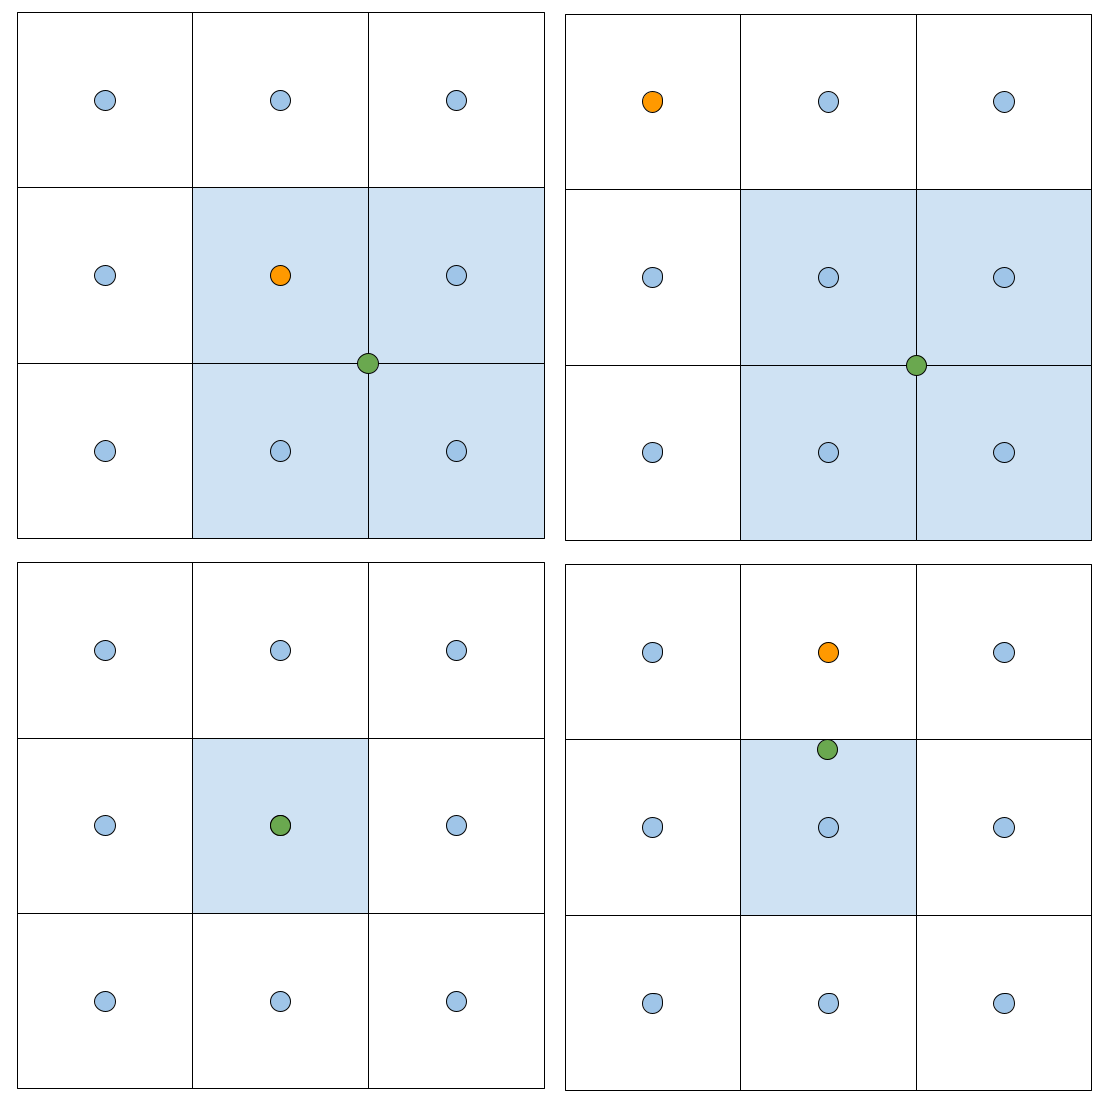
\includegraphics[width=0.5\linewidth]{../common/04_results/resources/detektion_min_und_max_fehler.png}
    \end{center}
    \caption{
        Extremsituationen zum Vergleich der Referenzposition und der wahren Position des Kugelmittelpunktes.
        Abgebildet ist ein Bildausschnitt mit 9 Pixeln. Die blauen Punkte sind die Pixelzentren, grün ist die wahre Position (subpixelgenau), orange ist die Referenzposition aus den Referenzdaten.
        Die Pixel rund um die wahre Position sind blau hinterlegt.
        Oben-Links: Der maximale Fehler ist eine halbe Pixeldiagonale, wenn die wahre Position zwischen vier Pixeln liegt und die Referenzposition einem der Pixel rund um die tatsächliche Position entspricht.
        Unten-Links: Der minimale Fehler ist $0$, wenn die wahre Position genau dem Pixelzentrum entspricht und dieses Pixel in den Referenzdaten ausgewählt wurde.
        Oben-Rechts: Der maximale Fehler ist 1.5 Pixeldiagonalen, wenn die wahre Position zwischen vier Pixeln liegt und die Referenzposition um ein Pixel daneben ist.
        Unten-Rechts: Der minimale Fehler ist eine halbe Pixelbreite/-höhe, wenn die wahre Position innerhalb des zentralen Pixels liegt und die Referenzposition um ein Pixel daneben ist.
    }
    \label{fig:detektion_resultate_min_max_fehler_referenzdaten}
\end{figure}

In Abschnitt \ref{kap:tracking} wurde beschrieben, dass in der Live-Detektion eine Stabilisierung der detektierten Positionen
über die Zeit durchgeführt wird.
In diesem Kapitel wurden nur Bilder für den Vergleich zwischen Detektion und Realität verwendet, wodurch es sich um Momentaufnahmen handelt.
Es kann sein, dass die Stabilisierung in gewissen Fällen die detektierten Positionen verbessert,
weil Positionsfehler in einzelnen Bildern geglättet werden.

\subsection{Performanz der Live-Detektion}
Die Performanz der Detektion ist für das Tracking und die Anzeige der Kugelpositionen in Echtzeit relevant.
Zur Messung wurde die Detektion 50-mal abwechselnd auf 24 Testbildern ausgeführt und die benötigte Zeit gemessen.
Dadurch wurden $50 \cdot 24 = 1200$ Detektionen ausgeführt.
Ausgeführt wurde dieser Test auf einem vierjährigen Laptop vom Modell Acer Aspire V 15 Nitro mit
einem Intel(R) Core(TM) i7-7700HQ CPU @ 2.80GHz und 16GB RAM.

Aufgrund dieses Tests konnte die durchschnittliche Dauer eines Detektionsdurchlaufs berechnet werden.
Diese beträgt 43.8ms und entspricht damit einer Framerate von 22.8 fps (frames per second).
Mit der aktuell eingesetzten Kamera, einer Intel RealSense D435 \cite{project2:aufbau}, kann mit der verwendeten Auflösung eine Framerate von
30 fps erreicht werden.
Mit dieser Performanz werden dementsprechend einzelne Frames übersprungen.
Die erreichte Performanz reicht allerdings aus, um Kugeln bei mittleren Geschwindigkeiten mit einer kleinen Verzögerung
zu verfolgen, siehe Abbildung \ref{fig:detection_delay}.

\begin{figure}[h!]
    \begin{center}
        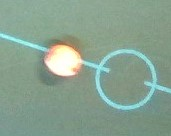
\includegraphics[width=0.4\linewidth]{../common/04_results/resources/detection_delay.jpg}
    \end{center}
    \caption{
        Sichtbare Verzögerung in der Detektion (vergrösserter Bildausschnitt).
        Die vergangene Zeit zwischen Bildaufnahme und Anzeige des Kreises um die detektierte Kugelposition herum ist zu gross,
        um die rollende Kugel perfekt zu verfolgen.
    }
    \label{fig:detection_delay}
\end{figure}

\subsection{Fehldetektionen an Armen und Händen}\label{kap:detektion_arme_haende}
Ein Problem der Live-Detektion ist, dass wenn ein Spieler mit der Hand in das Bild greift, um u.a. einen Stoss
durchzuführen, dann werden bei der Hand ebenfalls Kugeln detektiert, siehe Abbildung \ref{fig:detection_hand_problem}.
Dies ist darauf zurückzuführen, dass die Detektion eine Segmentierung des HSV-Farbraumes durchführt \cite{project2:snooker_detection}
und anschliessend darauf den Circle Hough transform \cite{wiki:circle_hough} ausführt.
Dadurch werden Kleider oder Haut ebenfalls als Bereiche erkannt, wo eine Kugel sein könnte.
Der Circle Hough transform findet anschliessend aufgrund von Kanten in diesen Bereichen Kreise,
welche dann als detektierte Kugeln übernommen werden.

\begin{figure}[h!]
    \begin{center}
        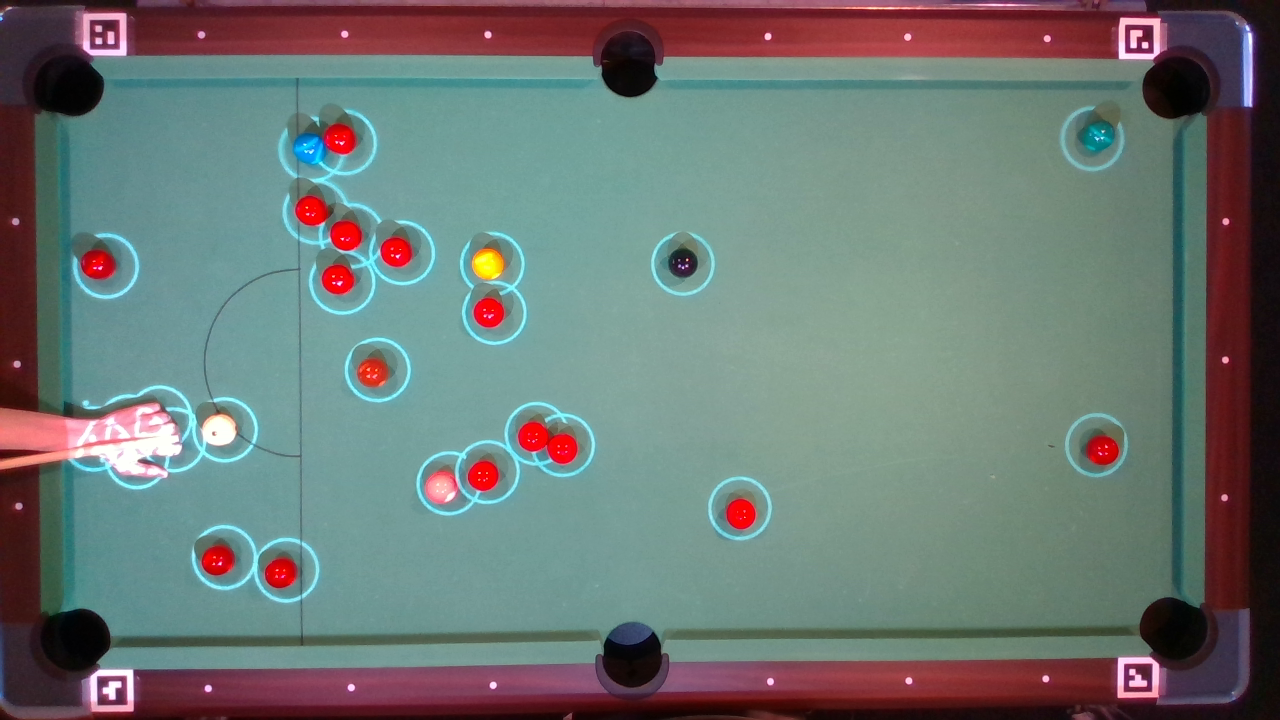
\includegraphics[width=0.8\linewidth]{../common/04_results/resources/detektierte_kugeln_auf_der_hand.png}
    \end{center}
    \caption{Fälschlich detektierte Kugeln auf der Hand}
    \label{fig:detection_hand_problem}
\end{figure}

Sofern die Arme und Hände des Spielers segmentiert werden könnten, wäre es möglich diese Fehler in der Detektion zu verhindern.
Dazu würden die segmentierten Regionen, wo eine Hand oder ein Arm abgebildet ist, in der Detektion ignoriert.
Diese Segmentation ist allerdings schwierig durchzuführen, da diese stark von Hautfarbe und Bekleidung abhängt.
Es wäre hier denkbar, ein vortrainiertes neuronales Netzwerk zu verwenden, welches eine Handsegmentation oder -detektion machen kann.

Die detektierten Kreise bei Armen und Händen sind mehrheitlich aus kosmetischen Gründen störend und könnten den Spieler ablenken.
Eine Suche sollte zum Zeitpunkt, da der Spieler gerade dabei ist, einen Stoss auszuführen, nicht durchgeführt werden.
Daher sind diese Fehldetektionen für die Suche irrelevant.

\newpage
\section{Tracking und Stabilisierung der Kugelpositionen}
Das in Abschnitt \ref{kap:tracking} beschriebene Tracking zur Stabilisierung der Kugelpositionen hat zu einer deutlichen,
visuellen Verbesserung der Live-Detektion und -Anzeige geführt.
Sofern der Spielstand ruhig ist, also keine Kugeln in Bewegung sind, bewegen sich die
projizierten Kreise rund um die detektierte Position kaum noch.
Ohne Tracking ist das Rauschen in der detektierten Position anhand der bewegenden Kreise sichtbar.

Diese visuelle Verbesserung kann auch statistisch quantifiziert werden, indem die Detektion auf einem Video eines
ruhigen Spielstandes durchgeführt wird. Die Detektion kann auf jedem einzelnen Frame des Videos durchgeführt werden, und
die detektierte Position mit derjenigen im vorherigen Frame verglichen werden.
Die Distanz zwischen der detektierten Position in Frame $F_{t-1}$ und derjenigen in Frame $F_{t}$ bildet anschliessend
eine Messung, die gesammelt wird.

Auf den gesammelten Distanzen können anschliessend statistische Kennzahlen berechnet werden.
Diese Messungen wurden mit und ohne Stabilisierung der Kugelpositionen durchgeführt, die Resultate sind in Tabelle \ref{tab:detektion_resultate_tracking_stats} aufgeführt.
Die Messungen basieren auf einem Videoausschnitt von 178 Frames eines Videos mit einem Spielstand von 21 stillstehenden Kugeln.
Die Messung wurde erst nach 30 Frames gestartet, damit die Messung mit eingeschalteter Stabilisierung bereits einige
Daten sammeln konnte.
Während dieser Aufwärmphase wäre die Detektion mit eingeschalteter Stabilisierung anfällig auf Rauschen in der Detektion,
wie es die Detektion ohne Stabilisierung ist.
Durch diesen Vorlauf von 30 Frames beträgt der gemessene Videoausschnitt 148 Frames.
Dies resultiert in $148 \cdot 21 = 3108$ Messwerten.
Aus Tabelle \ref{tab:detektion_resultate_tracking_stats} wird klar, dass die Stabilisierung die Bewegung der
detektierten Kugelpositionen deutlich verringern konnte.

\begin{table}[ht]
    \rowcolors{1}{\seccolor!10}{\seccolor!10} % Rows with 10% of secondary color
    \begin{tabular}{ lrr }
        \rowcolor{\seccolor!50}
        Bezeichnung & Stabilisierung ausgeschaltet & Stabilisierung eingeschaltet\\
        Anzahl Messwerte & 3108 & 3108\\
        Minimum & 0mm & 0mm\\
        Unteres Quartil $Q_{0.25}$ & 1.638916mm & 0.081972mm\\
        Median $Q_{0.5}$ & 2.359856mm & 0.129632mm\\
        Oberes Quartil $Q_{0.75}$ & 3.714067mm & 0.222898mm\\
        Quartilabstand $Q_{0.75} - Q_{0.25}$ & 2.075151mm & 0.140926mm\\
        Maximum & 13.590104mm & 4.043161mm\\
        Summe aller Messungen & 7654.91mm & 588.849mm
    \end{tabular}
    \caption{
        Statistische Zahlen zu der Verteilung der Veränderung der detektierten Kugelpositionen über eine Dauer von
        148 Video-Frames mit und ohne Stabilisierung.
        Bei einem Messwert handelt es sich um die Distanz zwischen der detektierten Kugelposition in Frame $F_{t-1}$
        und Frame $F_{t}$ für eine Kugel.
    }
    \label{tab:detektion_resultate_tracking_stats}
\end{table}
% ohne stabilisierung: Total delta movement summary: count=3108 min=0.000000, lower quartile=1.638916, median=2.359856, upper quartile=3.714067, max=13.590104
% mit  stabilisierung: Total delta movement summary: count=3108 min=0.000000, lower quartile=0.081972, median=0.129632, upper quartile=0.222898, max=4.043161
% ohne stabilisierung: Total delta movement: 7654.91mm, 148 frames, lost: 0
% mit  stabilisierung: Total delta movement: 588.849mm, 148 frames, lost: 0

In Abbildung \ref{fig:detektion_resultate_tracking_boxplot} sind die Daten aus Tabelle \ref{tab:detektion_resultate_tracking_stats}
in zwei Box-Plot-Diagrammen visualisiert.

\begin{figure}[h!]
    \begin{center}
        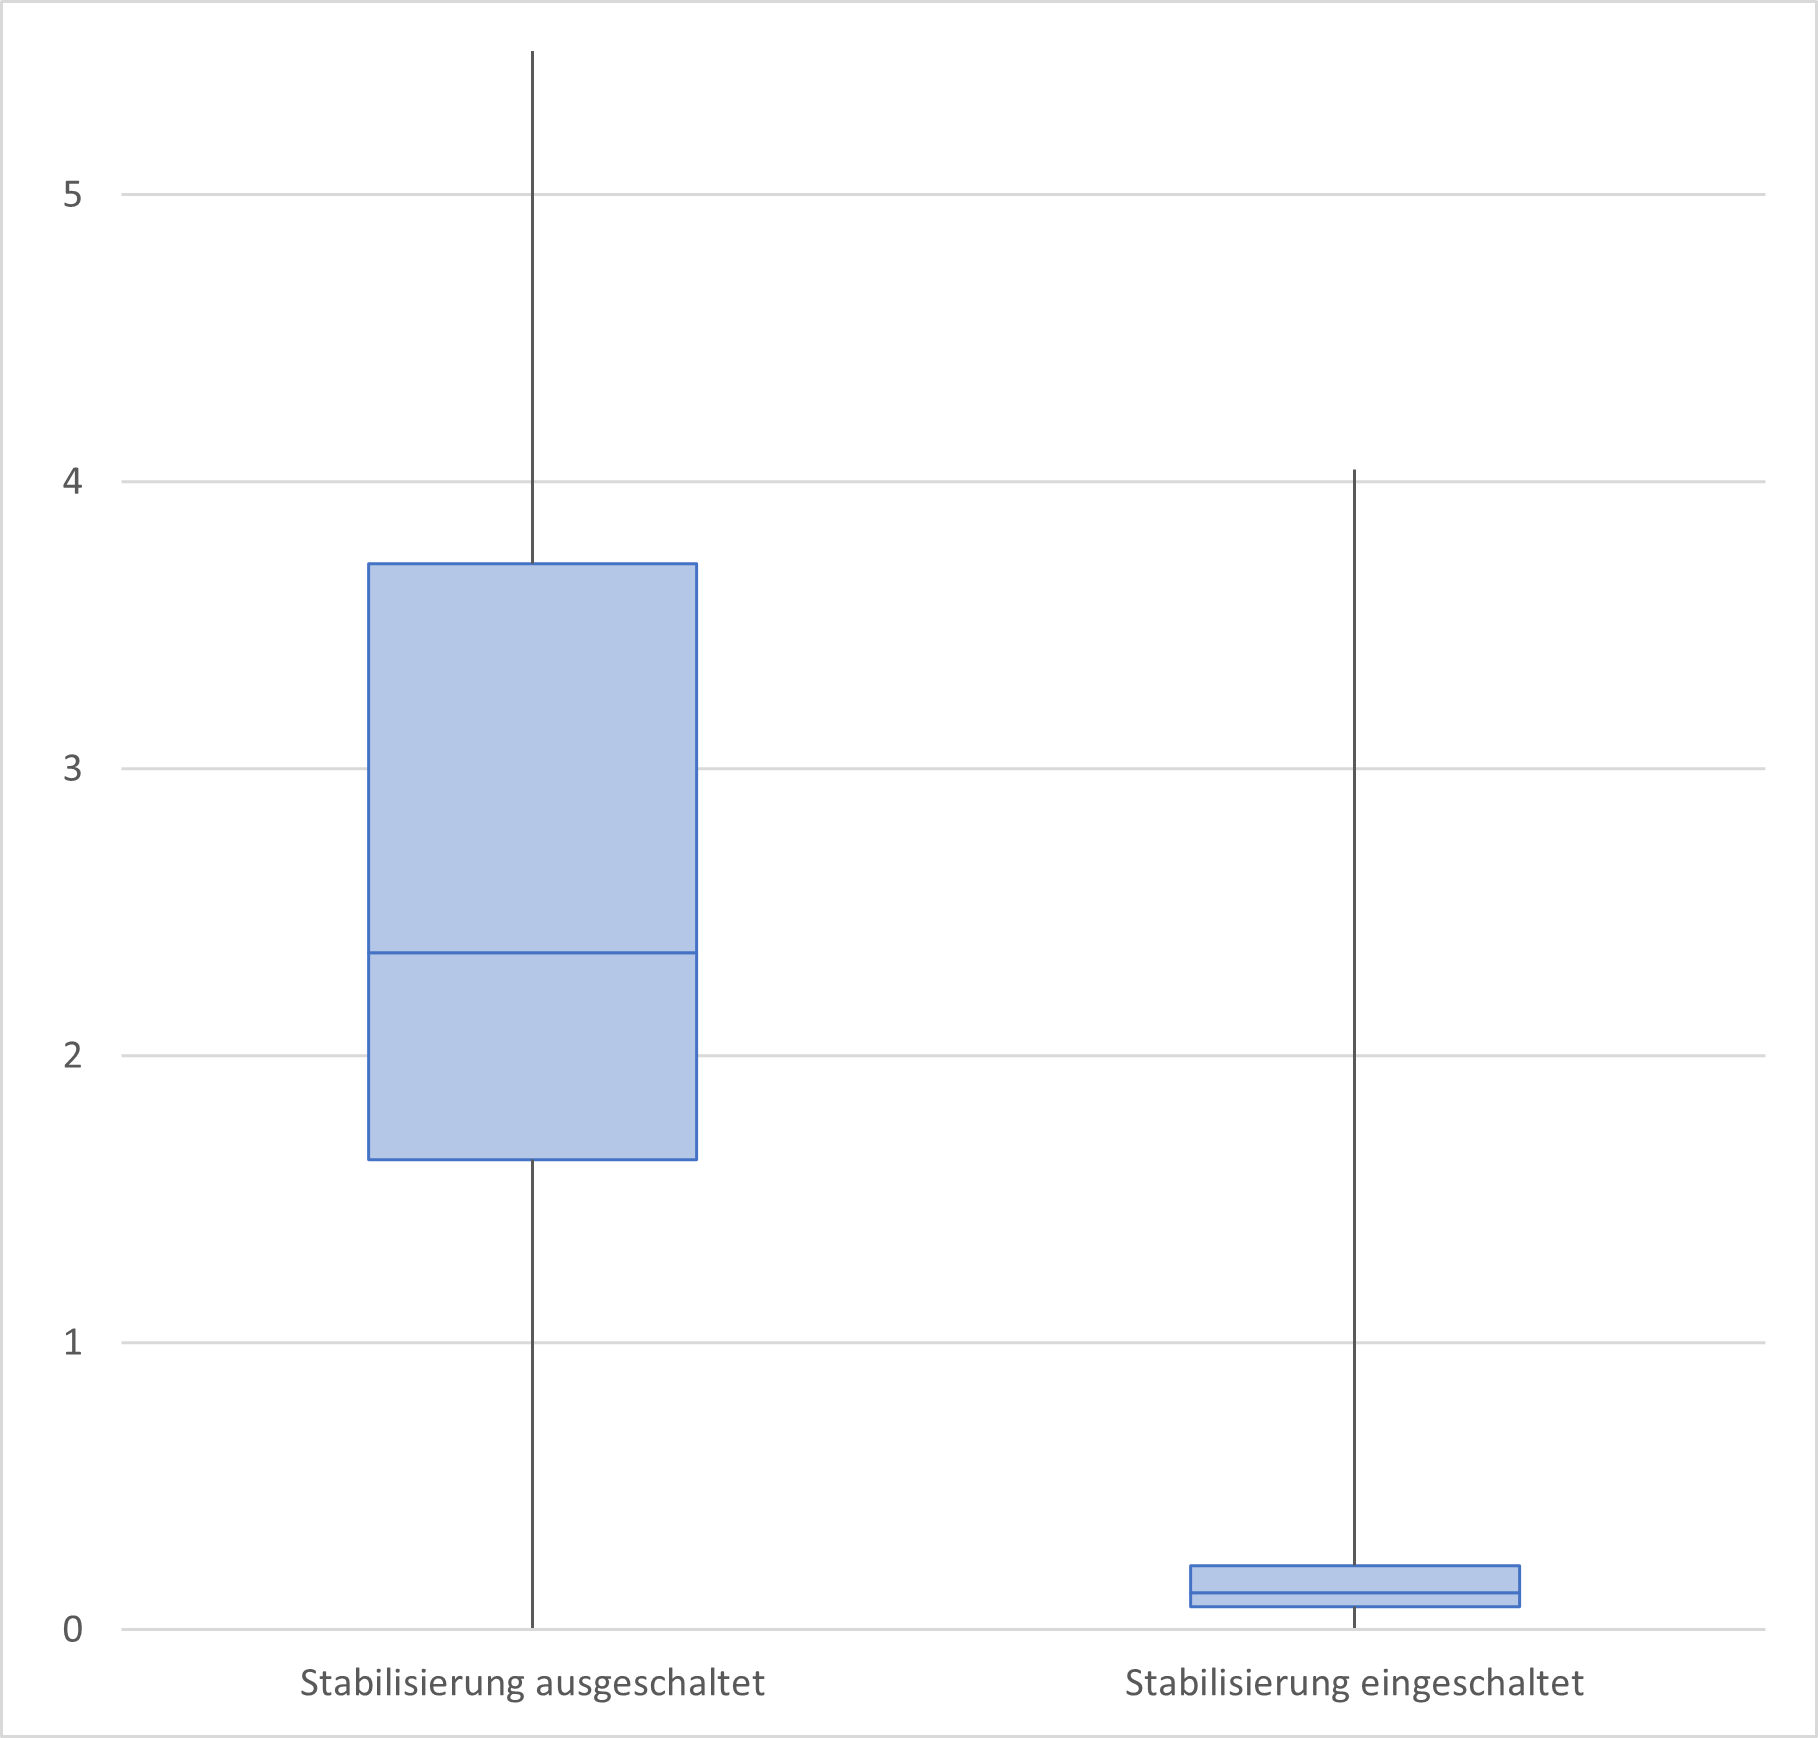
\includegraphics[width=0.5\linewidth]{../common/04_results/resources/stabilisierung_boxplot.png}
    \end{center}
    \caption{
        Box-Plot-Diagramme zu der Bewegung der Kugelpositionen mit und ohne Stabilisierung
        gemäss Tabelle \ref{tab:detektion_resultate_tracking_stats}.
        Der Wertebereich der Y-Achse wurde auf 5 beschränkt, damit das rechte Diagramm ersichtlich ist.
        Die Antenne des linken Diagrammes geht bis zum Maximum von 13.59mm.
    }
    \label{fig:detektion_resultate_tracking_boxplot}
\end{figure}

\section{Klassifikation}
Für die Beurteilung der Klassifikation, die in Kapitel \ref{kap:klassifikation} beschrieben wurde, wird eine
Wahrheitsmatrix\cite{wiki:confusion_matrix} (engl. \emph{confusion matrix}) verwendet.
Daraus können Metriken berechnet werden, welche eine Aussage über die Qualität der Klassifikation erlauben.

In Tabelle \ref{tab:klassifikation_resultate_confusion_matrix} ist die Wahrheitsmatrix der Testdaten
für die Klassifikation aufgeführt. Es wurden 32 Testbilder erstellt, wobei jeweils alle farbigen und einige rote Kugeln
auf jedem Bild abgebildet sind. Dies führt dazu, dass es mehr Testdaten für die roten Kugeln gibt als für die anderen farbigen Kugeln.
In den Testbildern sind keine Kugeln mit der Klasse \emph{unknown} vorhanden.

Aus der Wahrheitsmatrix ist ersichtlich, dass braune und rote Kugeln teilweise verwechselt werden.
Tatsächlich führt
% TODO: Bild mit Beispiel von braunen Kugeln, die wie rote aussehen
% TODO: weiter beschreiben
Die restlichen Kugelfarben werden sehr gut klassifiziert, lediglich ein Bild des Spielballs wird mit einer pinken Kugel verwechselt.
Keiner der Kugeln wurde die Klasse \emph{unknown} zugewiesen.

\begin{table}[ht]
\rowcolors{1}{\seccolor!10}{\seccolor!10} % Rows with 10% of secondary color
\begin{tabular}{ ccccccccccc }
        \rowcolor{\seccolor!50}
        &         & \multicolumn{9}{c}{\textbf{Wahre Farbe}}\\
        &         &   BROWN &    PINK &     RED &   BLACK &  YELLOW &   WHITE &    BLUE &   GREEN & UNKNOWN \\
        & BROWN   &      29 &       0 &      11 &       0 &       0 &       0 &       0 &       0 &       0 \\
        & PINK    &       0 &      32 &       0 &       0 &       0 &       1 &       0 &       0 &       0 \\
        & RED     &       3 &       0 &     213 &       0 &       0 &       0 &       0 &       0 &       0 \\
        & BLACK   &       0 &       0 &       0 &      32 &       0 &       0 &       0 &       0 &       0 \\
        & YELLOW  &       0 &       0 &       0 &       0 &      32 &       0 &       0 &       0 &       0 \\
        & WHITE   &       0 &       0 &       0 &       0 &       0 &      31 &       0 &       0 &       0 \\
        & BLUE    &       0 &       0 &       0 &       0 &       0 &       0 &      32 &       0 &       0 \\
        & GREEN   &       0 &       0 &       0 &       0 &       0 &       0 &       0 &      32 &       0 \\
        \multirow{-10}{*}{\rotatebox{90}{\textbf{Klassifizierte Farbe}}} & UNKNOWN &       0 &       0 &       0 &       0 &       0 &       0 &       0 &       0 &       0
\end{tabular}
\caption{Ergebnisse Klassifikation der Kugelfarben}
\label{tab:klassifikation_resultate_confusion_matrix}
\end{table}

% Total accuracy: 0.966518
% TODO: beschreiben

\subsection{Kandidatensuche}\label{sec:kandidatensuche}
Die Kandidatensuche, im Folgenden Suche genannt, wird über eine klassische Graphensuche durchgeführt, wobei der vollständige
Graph alle möglichen Stösse enthält.
Für die Suche gibt es zwei Möglichkeiten, entweder wird bei der weissen Kugel gestartet und von dort ein Stoss gesucht,
welcher eine andere Kugel ins Loch spielt, oder es wird bei einem oder mehreren Löchern gestartet und von dort ein Stoss gesucht,
welcher von der weissen Kugel ausgehend eine andere Kugel ins Loch spielt.

Nachfolgend wird die Rückwärtssuche beschrieben, welche ausgehend vom Zielloch startet, eine einzulochende Kugel findet
und anschliessend den Stoss bis zur weissen Kugel zurück sucht.
Dementsprechend ist der Root-Knoten des Suchbaumes das zu treffende Ziel (Loch).
Da ein handelsüblicher Billardtisch mehrere Löcher hat, muss pro Loch eine separate Suche durchgeführt werden.

Bei der Durchführung eines Expansionsschrittes werden ausgehend von einem Knoten im Suchbaum dessen Nachfolger-Knoten ermittelt.
Diese stellen im Fall vom Root-Knoten Kugeln dar, welche in dieses Loch gespielt werden könnten.
Aus diesen Kugeln werden Kugel-Knoten gebildet, welche diese Kugeln entweder auf direktem Wege oder indirekt über die Bande
in das Loch spielen lassen sollen.
Von diesen Kugel-Knoten startend, werden deren Nachfolger-Knoten in weiteren Expansionsschritten ermittelt, welche
wiederum Kugel-Knoten darstellen.
Diese Kugel-Knoten stellen dann Kugeln dar, welche die Kugel des Vorgänger-Kugel-Knotens entweder auf direktem Wege oder indirekt
über die Bande treffen sollen.
Sofern ein Kugel-Knoten die weisse Kugel darstellt, so ist dieser Kugel-Knoten ein Endzustand und damit ist der Stoss
über die Kette von Nachfolger- zu Vorgänger-Kugel-Knoten definiert.

Zur Veranschaulichung des Prinzips folgt ein Beispiel. Es wird vereinfacht angenommen,
dass der Tisch nur ein Loch hat. Für mehrere Ziele ergeben sich mehrere Suchbäume, einen pro Loch.
In Abbildung \ref{fig:backwardsearch_1} erfolgt die Eingabe des Suchalgorithmus in Form des Root-Knotens.
Es wird nur das zu treffende Ziel definiert.

\begin{figure}[h!]
    \begin{center}
        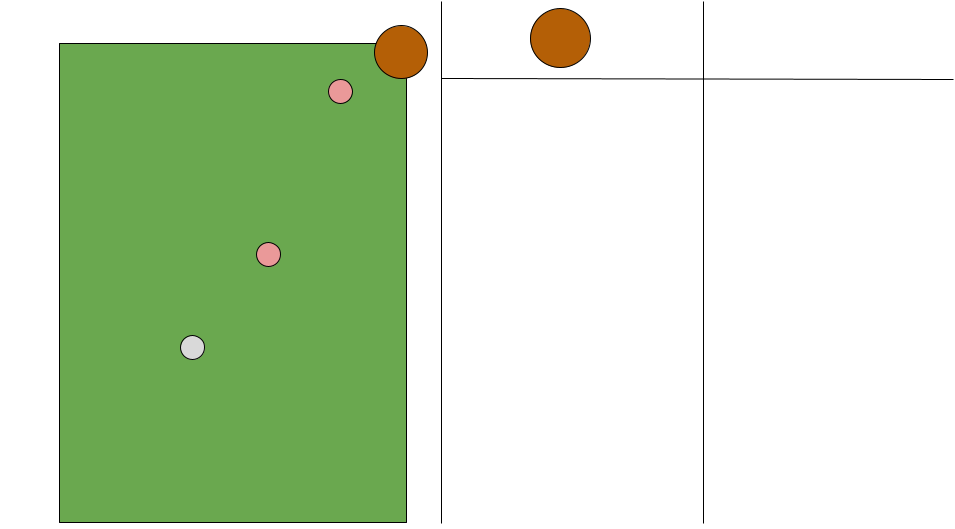
\includegraphics[width=0.5\linewidth]{../common/03_billiard_ai/resources/11_backwardsearch_1.png}
    \end{center}
    \caption{Kandidatensuche 1: Links ist der Spielstand auf dem Billardtisch abgebildet. Auf der rechten Seite des Tisches ist der Suchbaum dargestellt.
    Im ersten Schritt wurden ausgehend vom Zielloch noch keine Kugeln expandiert.
    Es stehen die beiden roten Kugeln zur Auswahl.}
    \label{fig:backwardsearch_1}
\end{figure}

In einem zweiten Schritt wird die einzulochende Kugel definiert. Es kommen lediglich die beiden roten Kugeln in Frage.
Nachfolgend wird der Pfad weiter betrachtet, bei dem die beim Loch näherstehende rote Kugel, gewählt wurde.
Abbildung \ref{fig:backwardsearch_2} zeigt, dass der Suchbaum um einen Knoten erweitert wurde.
\begin{figure}[h!]
    \begin{center}
        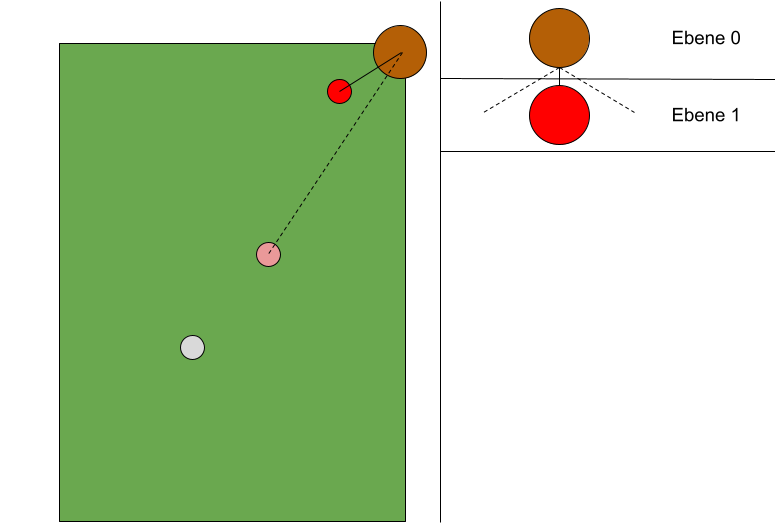
\includegraphics[width=0.5\linewidth]{../common/03_billiard_ai/resources/12_backwardsearch_2.png}
    \end{center}
    \caption{Kandidatensuche 2: Im ersten Expansionsschritt wurde die dunkelrot eingefärbte Kugel als einzulochende Kugel gewählt.
    Im Suchbaum ist diese dadurch als Knoten eingefügt worden. }
    \label{fig:backwardsearch_2}
\end{figure}

In Abbildung \ref{fig:backwardsearch_3} erfolgt der letzte Schritt. Hier sind verschiedene Optionen möglich, bspw.
könnte die weisse Kugel direkt oder über die Bande an die zuvor gewählte rote Kugel gespielt werden. Es könnte aber auch
die andere rote Kugel an die zuvor gewählte rote Kugel gespielt werden. Hier wird der Fall betrachtet, dass die weisse Kugel
indirekt über eine Bande an die zuvor gewählte rote Kugel gespielt wird.
\begin{figure}[h!]
    \begin{center}
        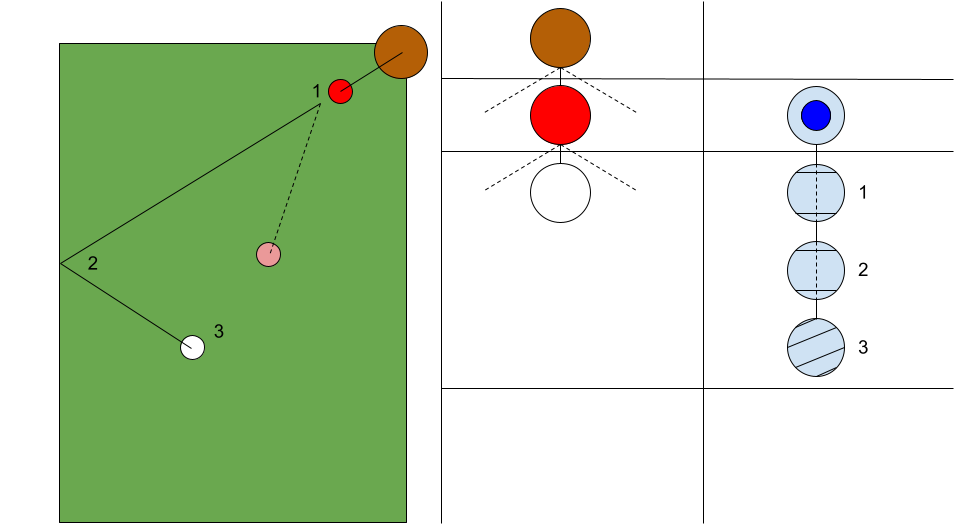
\includegraphics[width=0.5\linewidth]{../common/03_billiard_ai/resources/13_backwardsearch_3.png}
    \end{center}
    \caption{Kandidatensuche 3: Im letzten Expansionsschritt wurde die weisse Kugel gewählt und wird über die Bande an die rote Kugel gespielt.
    Der Suchbaum hat demnach einen neuen Knoten für die weisse Kugel, wodurch ein Pfad für einen vollständiger Stoss entstanden ist.}
    \label{fig:backwardsearch_3}
\end{figure}

Algorithmus \ref{alg:backward_search} verdeutlicht den Ablauf der \glqq Expand-Funktion\grqq. Zuerst wird eine
leere Liste namens \glqq nodes\grqq{} angelegt. Diese wird danach mit Nodes gefüllt, welche entweder durch einen Stoss
über eine weitere Kugel oder indirekt über die Bande zustande kommen. Die Nodes bilden das Ergebnis der Funktion.

\begin{algorithm}[H]
    \DontPrintSemicolon
    \SetKwFunction{expand}{expand}
    \SetKwProg{Fn}{Function}{}{}
    \Fn{\expand{node: Node, constantObjects: list} $\longrightarrow$ list[Node]}{
        nodes $\longleftarrow$ list()\\
        nodes $\longleftarrow$ append(expandBalls(node, constantObjects), nodes)\\
        nodes $\longleftarrow$ append(expandBank(node, constantObjects), nodes)\\
        \KwRet nodes
    }
    \caption{Algorithmus zur Durchführung eines Expansionsschritts bei der Kandidatensuche}
    \label{alg:backward_search}
\end{algorithm}

\subsubsection{Expansion einer Kugel}
In der anzuwendenden Graphensuche müssen die nächsten Knoten expandiert werden.
Eine Expansion kann über eine Kugel- oder über eine Bandenkollision stattfinden.

\paragraph{Expansion über eine Kugelkollision}\mbox{}\\

Bei einer Expansion einer Kugel wird der nächste Zielpunkt berechnet.
Das Prinzip wird in Abbildung \ref{fig:kugelexpansion} veranschaulicht.
Der Zielpunkt $T$, wohin die Kugel gespielt werden soll, ist bekannt.
Weiterhin ist die aktuelle Position $S$ der Kugel bekannt. Dazwischen kann der Vektor $\vec{d}$ gebildet werden.
\begin{align}
    \vec{d} = S - T
\end{align}
Damit die Kugel in Richtung des Zielpunkts $T$ rollt, muss diese von einer anderen Kugel am Punkt $Z$ angestossen werden.
Daher gilt es $Z$ zu bestimmen.
Der neue Zielpunkt $Z$ wird mithilfe des Vektors $d$ und dem bekannten Kugelradius $r$ berechnet.
\begin{align}
    Z = S + 2 \cdot r \cdot \hat{d}
\end{align}

\begin{figure}[h!]
    \begin{center}
        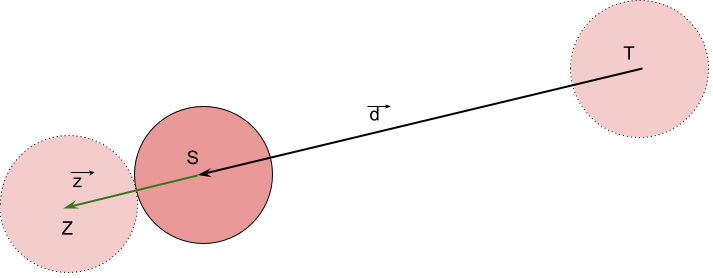
\includegraphics[width=0.5\linewidth]{../common/03_billiard_ai/resources/35_suchkandidat_kugel_expand.png}
    \end{center}
    \caption{Kugelexpansion}
    \label{fig:kugelexpansion}
\end{figure}

\paragraph{Expansion über eine Bandenkollision}\label{kandidatensuche:bandenkollisionstheorie}\mbox{}\\

Eine Kugel kann ebenso über eine oder mehrere Banden expandiert werden. Dazu muss bekannt sein, wie der Verlauf einer
Kugel nach einer Bandenkollision aussieht. Um diese Frage beantworten zu können, wurden zwei Arbeiten betrachtet.
Nach diesen Quellen gilt für den Stoss einer Kugel über die Bande, dass im Falle eines nicht vorhandenen Spins
der Ausfallswinkel dem Einfallswinkel entspricht. Dieses Verhalten wurde von den Autoren des Papers \glqq A theoretical analysis of billiard ball dynamics under cushion impacts\grqq{}
untersucht \cite{10.1243/09544062JMES1964}.
Der Abschnitt \glqq b\grqq{} der Abbildung \ref{fig:rail_rebound_angle_no_spin} zeigt die
funktionale fast lineare Abhängigkeit des Ausfallswinkels vom Einfallswinkel.
Diese Werte wurden anhand verschiedener Geschwindigkeiten in praktischen Experimenten ermittelt \cite{10.1243/09544062JMES1964}.

\begin{figure}[h!]
    \begin{center}
        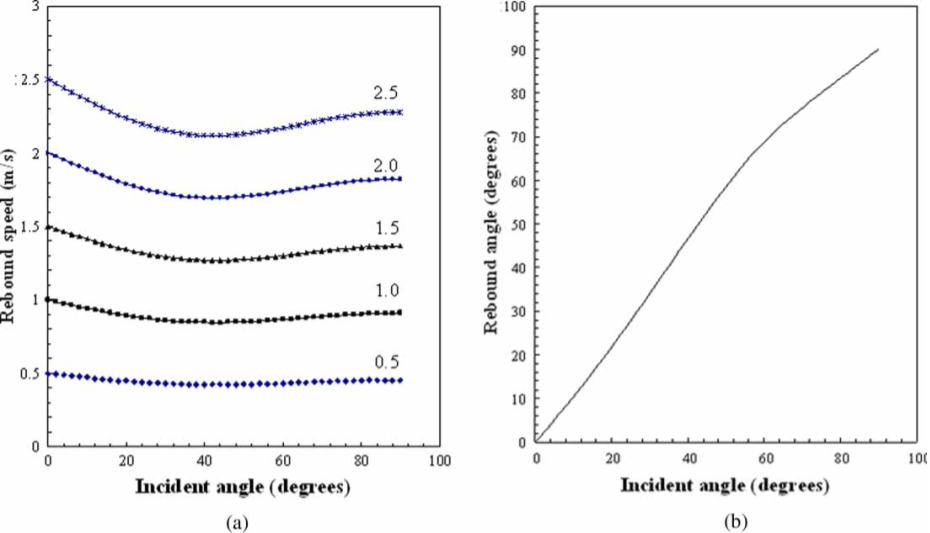
\includegraphics[width=0.5\linewidth]{../common/03_billiard_ai/resources/55_rail_rebound_angle_no_spin.png}
    \end{center}
    \caption{Geschwindigkeits- und Ausfallswinkelabhängigkeiten zum Einfallswinkel einer Kugel ohne Spin an einer Bande.
    Entnommen aus der Arbeit \cite{10.1243/09544062JMES1964} des Kapitels \glqq Results and Discussion\grqq. }
    \label{fig:rail_rebound_angle_no_spin}
\end{figure}

Eine weitere Bestätigung und eine ebenso ausführliche Behandlung des Themas findet sich im Buch \glqq The illustrated principles
of pool and billiards\grqq. Auch dieser Arbeit liegen praktische
\href{https://billiards.colostate.edu/high-speed-video/}{Experimente} zugrunde, die die Theorie bestätigen.
Grundsätzlich gilt das Prinzip 6.1 \glqq Bank shot geometry\grqq, welches besagt, dass
der Ausfallswinkel dem Einfallswinkel entspricht, dies ist
jedoch bei schwachen und starken wie auch bei Stössen der Bande sehr nahe liegenden Kugeln nicht korrekt \cite{book:the_ilustrated_principles_of_pool_and_billiards}.
So besagt das Prinzip 6.6 \glqq Rail throwback at high speed\grqq, dass der Ausfallswinkel kleiner wird, je stärker der Stoss ausgeführt wird.
Dieser Effekt tritt vor allem bei Einfallswinkeln zwischen $20^{\circ}$ und $50^{\circ}$ auf und ist auf
die seitliche Kompression der Bande zurückzuführen. Diese wird unterschiedlich stark eingedrückt und gibt durch die
darauffolgende Entspannung eine stärkere Kraft in die einfallende Richtung der Kugel zurück \cite{book:the_ilustrated_principles_of_pool_and_billiards}.
Dieser Umstand wird in der Abbildung \ref{fig:rebound_angle_no_spin_fast_shot} gezeigt.

\begin{figure}[h!]
    \begin{center}
        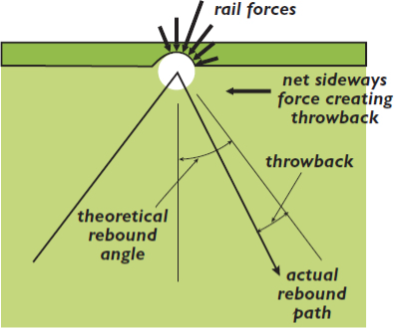
\includegraphics[width=0.3\linewidth]{../common/03_billiard_ai/resources/56_rebound_angle_no_spin_fast_shot.png}
    \end{center}
    \caption{Unterschiedliche Belastung der Bande bei starkem Stoss einer Kugel.
    Entnommen aus dem Buch \cite{book:the_ilustrated_principles_of_pool_and_billiards} des Kapitels \glqq 6 Bank and kick shots\grqq.}
    \label{fig:rebound_angle_no_spin_fast_shot}
\end{figure}

Trifft die Kugel langsam auf die Bande auf, so gilt Prinzip 6.7 \glqq Curved rebound path due to slow-speed roll\grqq.
Dieses verweist auf den Umstand, dass eine Kugel, die langsam auf die Bande trifft, aufgrund des resultierenden
Topspins kurvenförmig wegrollt. Der Effekt ist bei einem Einfallswinkel von $45^{\circ}$ am stärksten \cite{book:the_ilustrated_principles_of_pool_and_billiards}.
Die Abbildung \ref{fig:rebound_angle_no_spin_slow_shot} verdeutlicht das Prinzip.

\begin{figure}[h!]
    \begin{center}
        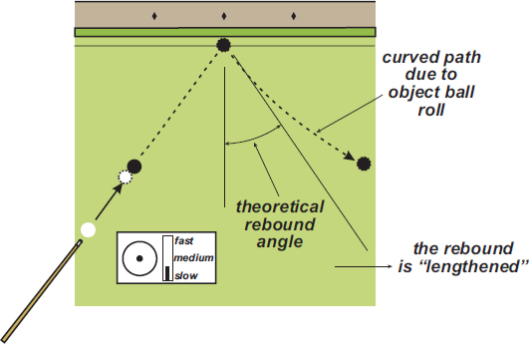
\includegraphics[width=0.4\linewidth]{../common/03_billiard_ai/resources/57_rebound_angle_no_spin_slow_shot.png}
    \end{center}
    \caption{Einfluss des Topspins auf den Ausfallswinkel bei schwachem Stoss einer Kugel an eine Bande.
    Entnommen aus dem Buch \cite{book:the_ilustrated_principles_of_pool_and_billiards} des Kapitels \glqq 6 Bank and kick shots\grqq.}
    \label{fig:rebound_angle_no_spin_slow_shot}
\end{figure}

Trifft eine Kugel langsam auf die Bande auf und ist sehr nahe, so dass sie zum Zeitpunkt der Kollision noch nicht zu rollen begonnen hat,
gilt Prinzip 6.8 \glqq Smaller rebound angle when close to the rail\grqq.
Dieses besagt, dass der Ausfallswinkel demnach kleiner wird \cite{book:the_ilustrated_principles_of_pool_and_billiards}.
Der resultierende Unterschied aufgrund der Distanzen wird in Abbildung \ref{fig:rebound_angle_no_spin_slow_shot_distance} veranschaulicht.

\begin{figure}[h!]
    \begin{center}
        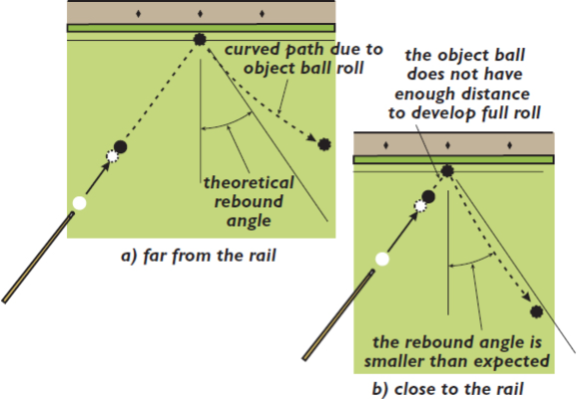
\includegraphics[width=0.4\linewidth]{../common/03_billiard_ai/resources/58_rebound_angle_no_spin_slow_shot_distance.png}
    \end{center}
    \caption{Einfluss der Distanz auf den Ausfallswinkel bei schwachem Stoss einer Kugel an eine Bande.
    Entnommen aus dem Buch \cite{book:the_ilustrated_principles_of_pool_and_billiards} des Kapitels \glqq 6 Bank and kick shots\grqq.}
    \label{fig:rebound_angle_no_spin_slow_shot_distance}
\end{figure}

\newpage
Aufgrund dieser Erkenntnisse und der gegebenen Abhängigkeit wird der Ausfallswinkel dem Einfallswinkel gleichgesetzt.
Technisch geschieht dies über einen geometrischen Ansatz durch eine Spiegelung \cite{math.stackexchange:1}
des Zielpunkts an der entsprechenden Bande, über welche gespielt werden soll.
In Abbildung \ref{fig:Tiefe über Bande erreichen mittels Reflektion} wird ein Suchschritt über eine Bande visualisiert.
Es wird ein Punkt $A$ an einer Bande gesucht, zu welchem die Kugel $B$ gespielt werden muss, um die Kugel $C$ zu treffen.
Dieser Bandenkollisionspunkt $A$ wird mithilfe eines Spiegelpunkts $\bar{C}$ des Punktes $C$ an der Bande berechnet.

\begin{figure}[h!]
    \begin{center}
        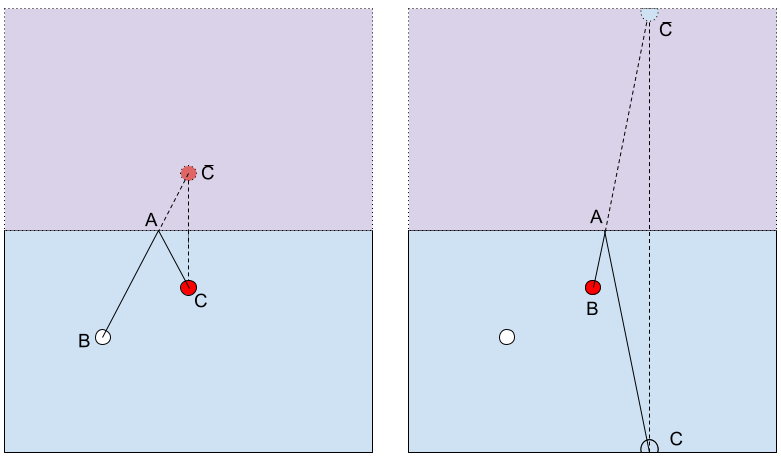
\includegraphics[width=0.5\linewidth]{../common/03_billiard_ai/resources/47_rail_reflection_1.png}
    \end{center}
    \caption{Zwei Fälle für ein Bandenspiel:
    Im ersten Fall wird für die weisse Kugel ein Kollisionspunkt an der oberen Bande bestimmt, um die rote Kugel zu treffen.
    Im zweiten Fall wird für die rote Kugel ein Kollisionspunkt an der oberen Bande bestimmt, um ins Ziel zu treffen.
    }
    \label{fig:Tiefe über Bande erreichen mittels Reflektion}
\end{figure}

Gegeben sind die folgenden Angaben (Parameter werden grossgeschrieben, Variablen dagegen klein):
\begin{align}
    B = \begin{pmatrix}B_X\\B_Y\end{pmatrix},
    C = \begin{pmatrix}C_X\\C_Y\end{pmatrix},
    \bar{C} = \begin{pmatrix}\bar{C_X}\\\bar{C_Y}\end{pmatrix},
\end{align}
Der Schnittpunkt kann über zwei Geraden berechnet werden, die über die Parameterform gegeben sind.
Eine dieser Geraden liefert der gespiegelte Punkt $\bar{C}$ mit $B$.
\begin{align}
    \vec{l} = \vec{\bar{C}} - \vec{B}\\
    L_1 = \vec{B} + \lambda_1 \cdot \vec{l}
\end{align}
Die andere Gerade ist über die Bande (Rail) gegeben, wobei $R_1$ der Startpunkt und $R_2$ der Endpunkt der Bande ist:
\begin{align}
    R_1 = \begin{pmatrix}R_{1X}\\R_{1Y}\end{pmatrix}, R_2 = \begin{pmatrix}R_{2X}\\R_{2Y}\end{pmatrix}\\
    \vec{r} = \vec{R_2} - \vec{R_1}\\
    L_2 = \vec{R_1} + \lambda_2 \cdot \vec{r}
\end{align}
Der Kollisionspunkt $A$ lässt sich über $\lambda_1$ der Gleichung \ref{eq:bandenkollisionspunkt} mithilfe der Linie $L_1$
bestimmen (Herleitung, siehe Anhang \ref{anhang:herleitung:bandenreflektion}).

\begin{align}
    \lambda_1 = \frac{r_x \cdot B_y - r_y \cdot B_x + R_{1,x} \cdot r_y - R_{1,y} \cdot r_x}{l_x \cdot r_y - \cdot l_y \cdot r_x}\label{eq:bandenkollisionspunkt}
\end{align}

Es gilt zu beachten, dass es sich bei der Billardkugel nicht um einen unendlich kleinen Punkt handelt und
daher deren Radius berücksichtigt werden muss.
Das Problem wird in Abbildung ~\ref{fig:bandenreflektion_kugelradius} dargestellt.
\begin{figure}[h]
    \begin{center}
        \includegraphics[width=0.5\linewidth]{../common/03_billiard_ai/resources/48_bandenreflektion_kugelradius.png}
    \end{center}
    \caption{Berücksichtigung des Kugelradius bei Bandenreflektion: Die Bande wird um den Kugelradius in Richtung Tischmitte verschoben.}
    \label{fig:bandenreflektion_kugelradius}
\end{figure}

Einerseits wird als Zielposition $C$ nicht die Kugelposition selbst, sondern ein um den Radius verschobener Punkt in
Gegenrichtung zur gewünschten Laufrichtung $\vec{r}$ der Kugel $C$ definiert. Andererseits wird die Bande, an welcher
gespiegelt wird, um den Radius der Kugel in Richtung des Zentrums verschoben. Die verschobene virtuelle Bande ist grün eingezeichnet.

Durch Studium mehrerer Beispiele wird ein allgemeiner Algorithmus hergeleitet. Hierbei wird das zuvor genannte Problem
mit dem Kugelradius vernachlässigt, da dieses durch die beschriebenen Positionskorrekturen behandelt werden kann.
Der Algorithmus kann unabhängig von dieser Korrektur beschrieben werden.

In einem ersten Schritt werden die Banden definiert, über welche der Zielpunkt gespiegelt werden soll. Dies sind in
diesem Beispiel die linke und die obere Bande, dementsprechend werden die grün markierten Spiegel zuerst links und
dann oben angewendet. Es resultieren die Punkte $\bar{C_0}$ und $\bar{C_1}$. Die Abbildung \ref{fig:zweifaches_bandenspiel_a} zeigt die
Situation mitsamt der gespiegelten Punkte.
\begin{figure}[h]
    \begin{center}
        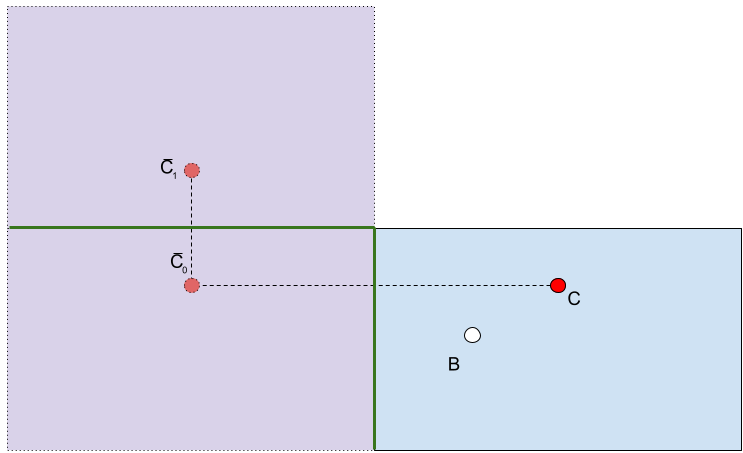
\includegraphics[width=0.5\linewidth]{../common/03_billiard_ai/resources/50_rail_reflection_2_a.png}
    \end{center}
    \caption{Zweifaches Bandenspiel - A: Der Zielpunkt C wurde zuerst an der linken, dann an der oberen Bande gespiegelt.}
    \label{fig:zweifaches_bandenspiel_a}
\end{figure}

Die Abbildung \ref{fig:zweifaches_bandenspiel_b} zeigt das Vorgehen, nachdem die Spiegelungen durchgeführt wurden.
Es wird der letzte Spiegelpunkt $\bar{C_n}$, in diesem Fall $\bar{C_1}$,
beibehalten, die Vorherigen werden verworfen. Vom Startpunkt $B$ aus wird eine Verbindung zum Spiegelpunkt $\bar{C_1}$
gezogen und alle Bandensegmente auf Schnittpunkte geprüft, was schliesslich im Punkt $A_0$ resultiert. Dies ist
der erste Kollisionspunkt mit der Bande und kann der Resultatsmenge hinzugefügt werden. Anschliessend wird der Spiegelpunkt
$\bar{C_1}$ an der Bande gespiegelt, an welcher der Kollisionspunkt liegt, in dem Fall an der Linken. Diese Spiegelung
resultiert im Spiegelpunkt $\bar{C_0}$.
\begin{figure}[h]
    \begin{center}
        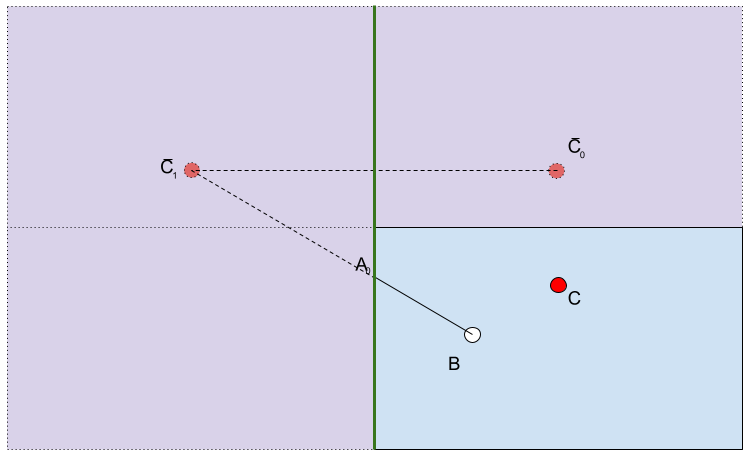
\includegraphics[width=0.5\linewidth]{../common/03_billiard_ai/resources/51_rail_reflection_2_b.png}
    \end{center}
    \caption{Zweifaches Bandenspiel - B: Der Schnittpunkt $A-0$ an der linken Bande ist der erste Bandenkollisionspunkt.
    Um den zweiten Bandenkollisionspunkt zu bestimmen, wird die Spiegelung an der linken Bande rückgängig gemacht.}
    \label{fig:zweifaches_bandenspiel_b}
\end{figure}

In der Abbildung \ref{fig:zweifaches_bandenspiel_c} ist der darauffolgende Schritt ersichtlich.
Es gibt zum Vorhergehenden keine wesentlichen Unterschiede.
Es wird wiederum nur der letzte Spiegelpunkt $\bar{C_0}$ beibehalten, zu welchem vom
neuen Startpunkt $A_0$ eine Verbindung gezogen wird.
Diese Halbgerade wird wiederum auf Schnittpunkte mit allen Bandensegmenten geprüft, was im Kollisionspunkt $A_1$ resultiert.
Dieser Kollisionspunkt wird der Resultatsmenge hinzugefügt und der Punkt $\bar{C_0}$
wird an der Bande mit dem Kollisionspunkt gespiegelt, in dem Fall der Oberen.
Diese Spiegelung überführt den Punkt $\bar{C_0}$ auf den ursprünglichen Punkt $C$, was das Ende des Algorithmus
bedeutet.
\begin{figure}[h]
    \begin{center}
        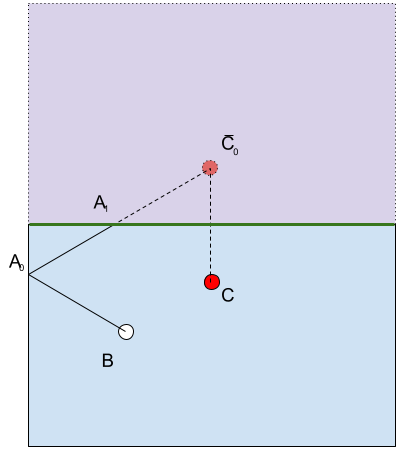
\includegraphics[width=0.5\linewidth]{../common/03_billiard_ai/resources/52_rail_reflection_2_c.png}
    \end{center}
    \caption{Zweifaches Bandenspiel - C: Der Schnittpunkt $A-1$ an der oberen Bande ist der zweite Bandenkollisionspunkt.
    Wenn die Spiegelung an der oberen Bande rückgängig gemacht wird, fällt der Zielpunkt wieder auf den ursprünglichen Punkt C zurück.}
    \label{fig:zweifaches_bandenspiel_c}
\end{figure}

Die Abbildung \ref{fig:zweifaches_bandenspiel_d} zeigt das endgültige Resultat, wenn der letzte Kollisionspunkt $A_1$
mit dem Zielpunkt $C$ verbunden wird.

\begin{figure}[h!]
    \begin{center}
        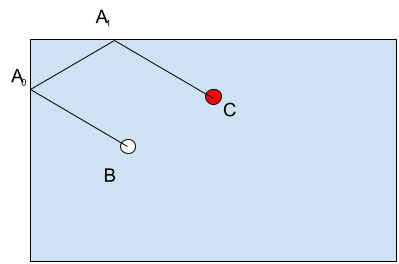
\includegraphics[width=0.5\linewidth]{../common/03_billiard_ai/resources/53_rail_reflection_2_d.png}
    \end{center}
    \caption{Zweifaches Bandenspiel - D: Die weisse Kugel wird von B über $A_0$ und $A_1$ an die rote Kugel an Position C gespielt.}
    \label{fig:zweifaches_bandenspiel_d}
\end{figure}

Dasselbe Prinzip kann auch auf ein Spiel über drei Banden angewendet werden, siehe Abbildung \ref{fig:Dreifache Reflektion an Banden}.
Es wird zuerst an der linken, dann an der oberen und anschliessend an der rechten Bande gespiegelt.
Es wird in einem Schritt wiederum der letzte Spiegelpunkt und dessen Startposition betrachtet, mit welchen der Kollisionspunkt
an einer Bande gefunden werden kann. Danach kann der Spiegelpunkt an dieser Bande gespiegelt werden und der nächste
Schritt kann starten. Dies wird so oft wiederholt, wie es Banden zum Spiegeln hat.
\begin{figure}[h]
    \begin{center}
        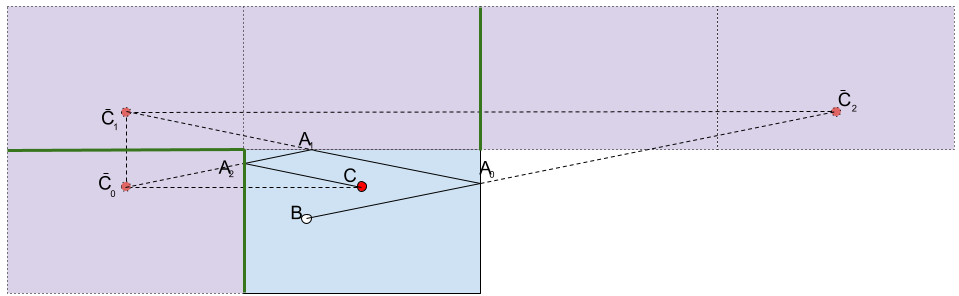
\includegraphics[width=1\linewidth]{../common/03_billiard_ai/resources/54_rail_reflection_3.png}
    \end{center}
    \caption{Dreifache Reflektion an Banden. Es wird zuerst an der linken, dann an der oberen und zuletzt an der rechten Bande gespiegelt.}
    \label{fig:Dreifache Reflektion an Banden}
\end{figure}

Eine Spiegelung kann durch die Anwendung der bandenspezifischen Transformationsmatrix $M$ erzielt werden, wobei $\vec{s}$
für den Spiegelvektor steht (Herleitung, siehe Anhang \ref{anhang:herleitung:bandenreflektion:zielpunkt}).
Hierbei steht der Punkt $C$ für den Zielpunkt, den es zu treffen gilt.
\begin{align}
    M = \begin{pmatrix}s_x & 0 & R^1_x - s_x \cdot R^1_x \\ 0 & s_y & R^1_y - s_y \cdot R^1_y \\ 0 & 0 & 1\end{pmatrix}\\
    \bar{C} = M \cdot C
\end{align}

Weiterhin stellt sich die Frage, an welcher Bande überhaupt gespiegelt werden darf.
Dazu wurden Definitionsbereiche für jede Bande erstellt, wie in Abbildung \ref{fig:Definitionsbereich_Bandenspiegelung} ersichtlich ist.
Punkte auf der roten Seite liegen ausserhalb des Definitionsbereichs, Punkte im grünen Bereich sind spiegelbar.
Des Weiteren ist die Bandennormale vorhanden, welche zum Ursprung des Koordinatensystems in der Tischmitte zeigt.

\begin{figure}[h!]
    \begin{center}
        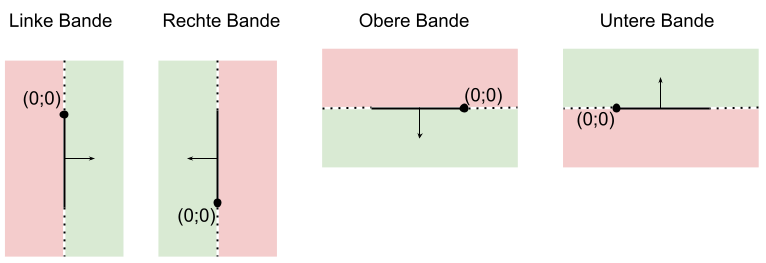
\includegraphics[width=1\linewidth]{../common/03_billiard_ai/resources/49_definitionsbereich_spiegelung_bande.png}
    \end{center}
    \caption{Definitionsbereich einer Bandenspiegelung. Wenn sich ein Zielpunkt im roten Bereich befindet, kann dieser nicht über die Bande angespielt werden.}
    \label{fig:Definitionsbereich_Bandenspiegelung}
\end{figure}

Um für einen Punkt $C$ herauszufinden, ob dieser spiegelbar ist, muss nur geprüft werden, ob er im Definitionsbereich liegt.
Dazu wird der Ursprung des Koordinatensystems zum Start der Bande verschoben und es wird die elementweise Multiplikation
des verschobenen Punktes $C'$ mit der Bandennormale durchgeführt.
Die Elemente des Vektors werden geprüft, ob sie grösser oder gleich dem Nullvektor sind.
Dies resultiert in einem Vektor, welcher eine $0$ speichert, wenn das Element kleiner und $1$, wenn es grösser ist.
Abschliessend wird die quadrierte Länge des resultierenden Vektors gebildet, diese Länge muss $2$ entsprechen, in dem
Fall liegt der Punkt im Definitionsbereich.
\begin{align}
    C^{'} = C \cdot T^0\\
    \bar{C} = C^{'} \cdot \hat{n}\\
    \vec{r} = \bar{C} \geq \vec{0}\\
    l = \vec{r} \cdot \vec{r}\\
    p = l == 2
\end{align}

Wird ein Punkt geprüft, der auf derselben Höhe wie eine Bande liegt, muss zusätzlich die jeweilige Komponente des Punktes
$\bar{C}$ grösser als $0$ sein, bei der die Komponente des Normalenvektors ungleich $0$ ist.

\clearpage
Algorithmus \ref{alg:stoss_ueber_bande_1} und \ref{alg:stoss_ueber_bande_2} zeigt, wie ein Stoss über die Bande gefunden werden kann.
Dazu werden in einem ersten Schritt alle möglichen Kombinationen der Banden gebildet, was auch den letzten Spiegelpunkt
$\bar{C_n}$ generiert. Danach können die Zielpositionen bestimmt werden, wobei auch geprüft wird, ob der Weg zwischen
den Positionen passierbar ist. Sollte dies nicht der Fall sein, wird dieser Lösungskandidat verworfen.

\begin{algorithm}[H]
    \DontPrintSemicolon
    \SetKwFunction{expandByRail}{expandByRail}
    \SetKwFunction{combos}{combos}
    \SetKwFunction{canReflect}{canReflect}
    \SetKwFunction{reflect}{reflect}
    \SetKwProg{Fn}{Function}{}{}
    \Fn{\expandByRail{B: vec2, C: vec2, reflections: int, rails: Rail[]} $\longrightarrow$ Node[]}{
        nodes $\longleftarrow$ Node[]\\
        combinations $\longleftarrow$ combos(reflections, C, rails)\\
        \For{combination in combinations}{
            targets $\longleftarrow$ target(B, C, combination.second,rails, combination.first)\\

            \If{! empty(targets)}{
                nodes $\longleftarrow$ append(physicalEvents(B, C, targets), nodes)
            }
        }
        \KwRet nodes
    }
    \;
    \Fn{\combos{reflections: int, target: vec2, rails: Rail[]} $\longrightarrow$ (Rail[], vec2)[]}{
        combinations: (Rail[], vec2, bool)[] $\longleftarrow$ []\\
        \For{rail in rails}{
            combinations $\longleftarrow$ append(([rail], reflect(target, rail), canReflect(target, rail)), combinations)
        }
        \For{index $\longleftarrow$ 1 < reflections}{
            \For{railIndex $\longleftarrow$ 0 < length(rails)}{
                rail $\longleftarrow$ rails[railIndex]\\
                \If{combinations[railIndex].third and canReflect(combinations[railIndex].second, rail)}{
                    combinations[railIndex].first $\longleftarrow$ append(rail, combinations[railIndex].first)\\
                    combinations[railIndex].second $\longleftarrow$ reflect(combinations[railIndex].second, rail)
                }
                \Else{
                    combinations[railIndex].third $\longleftarrow$ false
                }
            }
        }

        results: (Rail[], vec2)[] $\longleftarrow$ []\\
        \For{railIndex $\longleftarrow$ 0 < length(rails)}{
            \If{combinations[railIndex].third}{
                results $\longleftarrow$ append((combinations[railIndex].first, combinations[railIndex].second), results)
            }
        }

        \KwRet results
    }
    \;
    \Fn{\canReflect{C: vec2, rail: Rail} $\longrightarrow$ bool}{
        moved $\longleftarrow$ C $-$ rail.start\\
        reflected $\longleftarrow$ moved $\cdot$ rail.normal\\
        possible $\longleftarrow$ reflected $\geq \vec{0}$\\
        \KwRet possible $\cdot$ possible $= 2$
    }
    \;
    \Fn{\reflect{C: vec2, rail: Rail} $\longrightarrow$ vec2}{
        reflected: vec3 $\longleftarrow$ vec3(C, 1.0)\\
        \KwRet vec2(rail.M $\cdot$ reflected)
    }
    \caption{Algorithmus zur Berechnung eines Stosses über die Bande - Teil 1}
    \label{alg:stoss_ueber_bande_1}
\end{algorithm}
\newpage
\begin{algorithm}[H]
    \DontPrintSemicolon
    \SetKwFunction{target}{target}
    \SetKwProg{Fn}{Function}{}{}
    \Fn{\target{B: vec2, C: vec2, reflected: vec2, rails: Rail[], combo: Rail[]} $\longrightarrow$ vec2[]}{
        targets $\longleftarrow$ vec2[]\\
        start $\longleftarrow$ B\\
        \While{! empty(combo)}{
            comboRail $\longleftarrow$ pop(combo)\\
            target $\longleftarrow$ $(\infty, \infty)$\\
            \For{rail in rails}{
                railIntersection $\longleftarrow$ halfLineLineSegmentIntersection(start, (reflected - start), rail.start, rail.end)\\
                \If{railIntersection and start <> railIntersection}{
                    target $\longleftarrow$ railIntersection\\
                    reflected $\longleftarrow$ reflect(reflected, rail)\\
                    break
                }
            }
            \If{! shotPossible(start, target)}{
                \KwRet {}
            }
            targets $\longleftarrow$ append(target, targets)\\
            start $\longleftarrow$ target\\
        }

        If{! shotPossible(start, C)}{
            \KwRet {}
        }
        \KwRet targets
    }
    \caption{Algorithmus zur Berechnung eines Stosses über die Bande - Teil 2}
    \label{alg:stoss_ueber_bande_2}
\end{algorithm}

\paragraph{Prüfung der Ausführbarkeit eines Stosses}\mbox{}\\

Für die Expansion einer Kugel, sei es über eine weitere Kugel oder über eine Bande,
muss geprüft werden, dass keine weitere Kugel im Weg ist. Dies wird über die Berechnung
des Distanzvektors zwischen dem Vektor $\vec{d}$ und der zu prüfenden Kugel erzielt. Dasselbe Prinzip wird
in Kapitel \ref{kap:kugelkollision:performanceverbesserung} beim Fall einer dynamisch-statischen Kugelkollision erläutert.

%Bei der Prüfung auf eine mögliche Bandenkollision zwischen der aktuellen Position und dem Zielpunkt muss der Durchmesser
%der Kugel mitberücksichtigt werden. Eine mögliche Situation wird in Abbildung \ref{fig:kugelexpansion_bandenkollision} dargestellt.
%Dazu die Bande $R$ in Normalenrichtung verschoben, wobei die Normale in Richtung des Koordinatenursprungs zeigt. Es resultiert
%die virtuelle Bande $R_V$. Da die Bande durch zwei Punkte (Start und Ende) definiert ist, kann eine Gerade beschrieben werden.
%Dies gilt ebenso für die Kugel $K_1$. Deren Geradengleichung lautet:
%\begin{align}
%    K_1(\lambda) = S - \lambda \cdot \hat{d}
%\end{align}
%Ein Schnittpunkttest zwischen diesen Geraden sollte kein Ergebnis liefern, ansonsten wird vor dem Erreichen des Zielpunkts
%$T$ eine Kollision mit der Bande stattfinden, wie es in diesem Szenario der Fall ist.

%\begin{figure}[h!]
%    \begin{center}
%        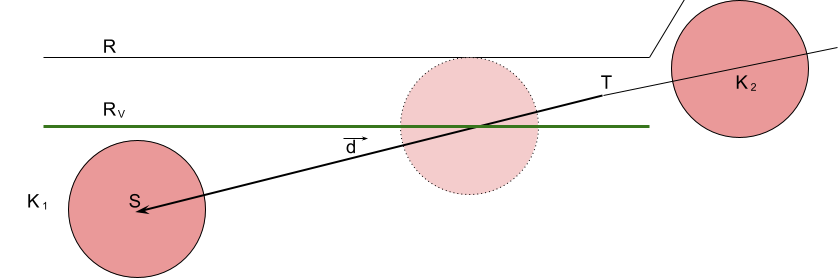
\includegraphics[width=0.5\linewidth]{../common/03_billiard_ai/resources/36_suchkandidat_kugel_expand_banden_kollision.png}
%    \end{center}
%    \caption{Kugelexpansion - Bandenkollision}
%    \label{fig:kugelexpansion_bandenkollision}
%\end{figure}

Sobald die weisse Kugel expandiert wird, muss sichergestellt werden, dass diese auch an der entsprechenden Position
mit dem Queue getroffen werden kann.
Dies wird, wie in Abbildung \ref{fig:kugelexpansion_platz_fuer_queue} veranschaulicht,
durch einen Vektor $\vec{s}$ mit einer bestimmten Länge $s$ entgegen der Rollrichtung der Kugel sowie einem Mindestabstand
$e$ zu diesem Vektor sichergestellt. Die Länge von $e$ wird auf $10 [mm]$ gewählt. Von jeder Kugel aus
werden die Abstände gemessen, liegt die Kugel zwischen $W$ und $W + \vec{s}$, so wird der Abstand senkrecht zum Vektor $\vec{s}$
berechnet, zu sehen bei der Kugel $K_1$. Liegt die Kugel wie $K_2$ vorne oder hinten, wird der Abstand zum Punkt $W$ oder $W + \vec{s}$
berechnet. Für die so erhaltenen Distanzen $d_i$ muss gelten, wobei $r$ für den Kugelradius steht:
\begin{align}
    d_i >= e + r
\end{align}

Liegt die Kugel in Richtung der Rollrichtung, wurde die Bedingung bereits geprüft, ansonsten dürfte die weisse Kugel nicht
expandiert worden sein. Daher muss dieser Fall nicht speziell behandelt werden.

\begin{figure}[h!]
    \begin{center}
        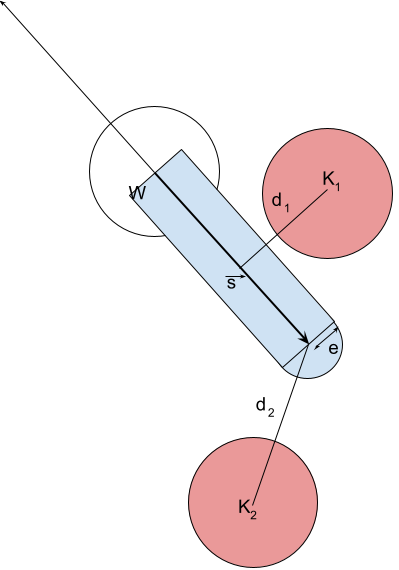
\includegraphics[width=0.3\linewidth]{../common/03_billiard_ai/resources/37_platz_fuer_queue.png}
    \end{center}
    \caption{Kugelexpansion - Platz für Queue. Der blau hinterlegte Bereich hinter der weissen Kugel darf nicht von anderen Kugeln belegt sein,
        damit diese mithilfe des Queues wie gewünscht angestossen werden kann.}
    \label{fig:kugelexpansion_platz_fuer_queue}
\end{figure}

\newpage
\subsubsection{Bewertungsfunktion}
Um die Suche zu vereinfachen und in eine spezifische Richtung zu lenken, wo die besten Resultate zu erwarten sind, ist
es unerlässlich eine Bewertung des Stosses durchzuführen.
Die Bewertungsfunktion wurde so definiert, dass sie sich auf den aktuell expandierten Knoten beschränkt.
Die Kosten für eine Expansion werden über die Pfade aufsummiert.
Anhand der Summen kann jeweils der kostengünstigste Pfad evaluiert und verfolgt werden.
Abbildung \ref{fig:suchbaum_bewertung} zeigt das Prinzip.
Dieses Vorgehen entspricht demjenigen des Dijkstra-Algorithmus \cite{wiki.dijkstra:1}.
\begin{figure}[h!]
    \begin{center}
        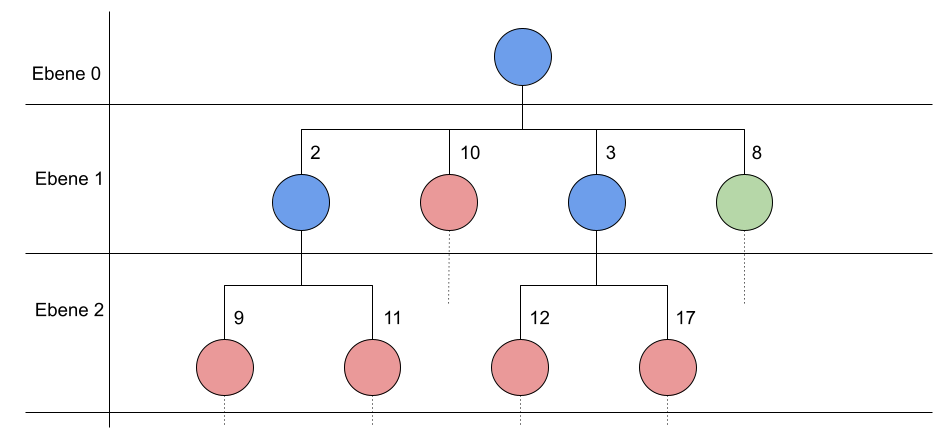
\includegraphics[width=0.8\linewidth]{../common/03_billiard_ai/resources/28_suchbaum_bewertung.png}
    \end{center}
    \caption{Bewertung eines Suchbaums: Die Knoten werden je nach Bedeutung mit unterschiedlichen Farben markiert.
    Wenn sie bereits expandiert wurden, sind sie blau. Grün, wenn der Knoten im nächsten Schritt expandiert wird,
    da er die geringsten Pfadkosten aufweist und rot, wenn der Knoten nicht in Frage kommt aufgrund zu hoher Kosten.}
    \label{fig:suchbaum_bewertung}
\end{figure}

Die Kosten werden auf Basis dreier Kriterien\footnote{Die Kriterien Distanz und Winkel werden wie
in Publikation \cite{inproceedings:billiard_ai:1} verwendet.} gebildet:
\begin{enumerate}
    \item Die \emph{Distanz}, welche eine Kugel zurücklegt.
    \item Der \emph{Winkel}, in welcher ein Zielpunkt getroffen werden muss.
    \item Die \emph{Indirektion}, wenn eine Kugel über die Banden oder über eine andere Kugel angestossen wird.
\end{enumerate}

Jeder dieser Werte liegt zwischen $0$ und $1$.
Die ersten beiden Kriterien sind in Abbildung \ref{fig:suche_knoten_expansionskosten} dargestellt.
Es werden zwei Expansionen gezeigt.
Die relevanten Informationen $d$ für die Distanz sowie $\alpha$ für den Winkel weisen
einen entsprechenden Index auf, welcher den Expansionsschritt markiert.
Beim ersten Expansionsschritt bildet der Zielpunkt
den Elternknoten.
Der Winkel $\alpha_1$ ist definiert durch die Rollrichtung der Kugel und einer Normalen auf den Zielpunkt.
Die Normalen zeigen jeweils zum Ursprung in der Mitte des Tisches.
Die Distanz $d_1$ ist definiert über die Länge des zurückzulegenden Weges.
Ist in einem Expansionsschritt die weisse Kugel betroffen, werden die Distanzkosten mit den
Distanzkosten des vorangegangenen Expansionsschritts gewichtet.
Dies stellt sicher, dass der Weg, welcher die nächste Kugel nehmen wird, möglichst kurz sein muss,
damit sich ein allfälliger Fehler beim Stoss der weissen Kugel nicht zu stark akkumuliert.
Im zweiten Fall wird der Winkel $\alpha_2$ durch die Rollrichtung der ersten und der Rollrichtung der zweiten Kugel definiert.

\begin{figure}[h!]
    \begin{center}
        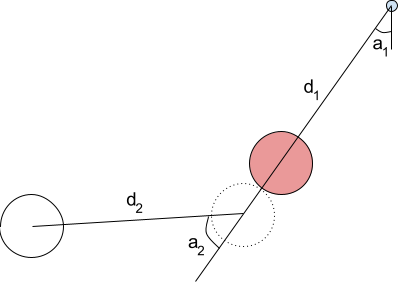
\includegraphics[width=0.4\linewidth]{../common/03_billiard_ai/resources/29_suchbaum_expansionskosten.png}
    \end{center}
    \caption{Zusammensetzung der Kosten eines Stosses:
    Die Kugeln müssen die Distanzen $d_1$ und $d_2$ zurücklegen.
    Die rote Kugel muss im Winkel $\alpha_1$ getroffen werden.
    Die rote Kugel wird dadurch im Winkel $\alpha_2$ in das Zielloch gespielt.
    Der Vektor $\vec{n}$ ist die Normale des Ziellochs, welche für die Berechnung des Winkels $\alpha_2$ verwendet wird.
    }
    \label{fig:suche_knoten_expansionskosten}
\end{figure}

Um die beiden Grössen vergleichen zu können, müssen sie in dieselbe Grössenordnung gebracht werden. Aus diesem Grund
werden sie durch die maximal möglichen Werte normiert \cite{qucosa:ein_billardroboter:1}. Für die Distanz ist dies die
Diagonale über den Tisch, für den Winkel wird ein maximal möglicher Wert von $87^\circ$ gewählt, dies ist bereits bei
der Suche berücksichtigt. Es gilt die Annahme, dass je kürzer der Weg und je kleiner der Winkel,
desto einfacher der Stoss.
\begin{align}
    d_{krit} = \frac{d_i}{d_{max}}\\
    \alpha_{krit} = \frac{\alpha}{\alpha_{max}}
\end{align}
Aktuell fliesst der Winkel $\alpha_{krit}$ zu stark in die Bewertung ein. Daher wird dieser durch eine kubische
Bézier-Kurve \cite{wiki.bezier:1} gewichtet. Die Parameter lauten wie folgt.
\begin{align}
    P_0 = \begin{pmatrix} 0 & 0\end{pmatrix}\\
    P_1 = \begin{pmatrix} 1 & 0\end{pmatrix}\\
    P_2 = \begin{pmatrix} 0.5 & 1\end{pmatrix}\\
    P_3 = \begin{pmatrix} 1 & 1\end{pmatrix}\\
    P = \begin{pmatrix} P_0 \\ P_1 \\ P_2 \\ P_3\end{pmatrix}\\
    T = \begin{pmatrix} t^3 & t^2 & t & 1\end{pmatrix}\\
    M = \begin{pmatrix}
            -1 &  3 & -3 & 1\\
             3 & -6 &  3 & 0\\
            -3 &  3 &  0 & 0\\
             1 &  0 &  0 & 0
        \end{pmatrix}\\
    \alpha^G_{krit} = f(t = \alpha_{krit}) = T \cdot M \cdot P
\end{align}
Nach dieser Gewichtung resultiert ein Punkt im zweidimensionalen Raum, wovon die y-Komponente als $\alpha^G_{krit, y}$ verwendet wird.
Die Kurve ist in Abbildung \ref{fig:suche_knoten_gewichtung_winkelkosten}
visualisiert. Es wird deutlich, dass kleinere Winkel einen eher geringen Einfluss auf die Kosten haben.
Ab einem Winkel von $50^\circ$, welcher auf der Grafik \ref{fig:suche_knoten_gewichtung_winkelkosten} als Punkt $D_1$ markiert ist,
beginnt die Kurve bis etwa $80^\circ$ stark zu steigen.
Ab dort flacht sie wiederum ab, bis die Kosten von $90^\circ$ schliesslich den Wert $1$ erreichen.

\begin{figure}[h!]
    \begin{center}
        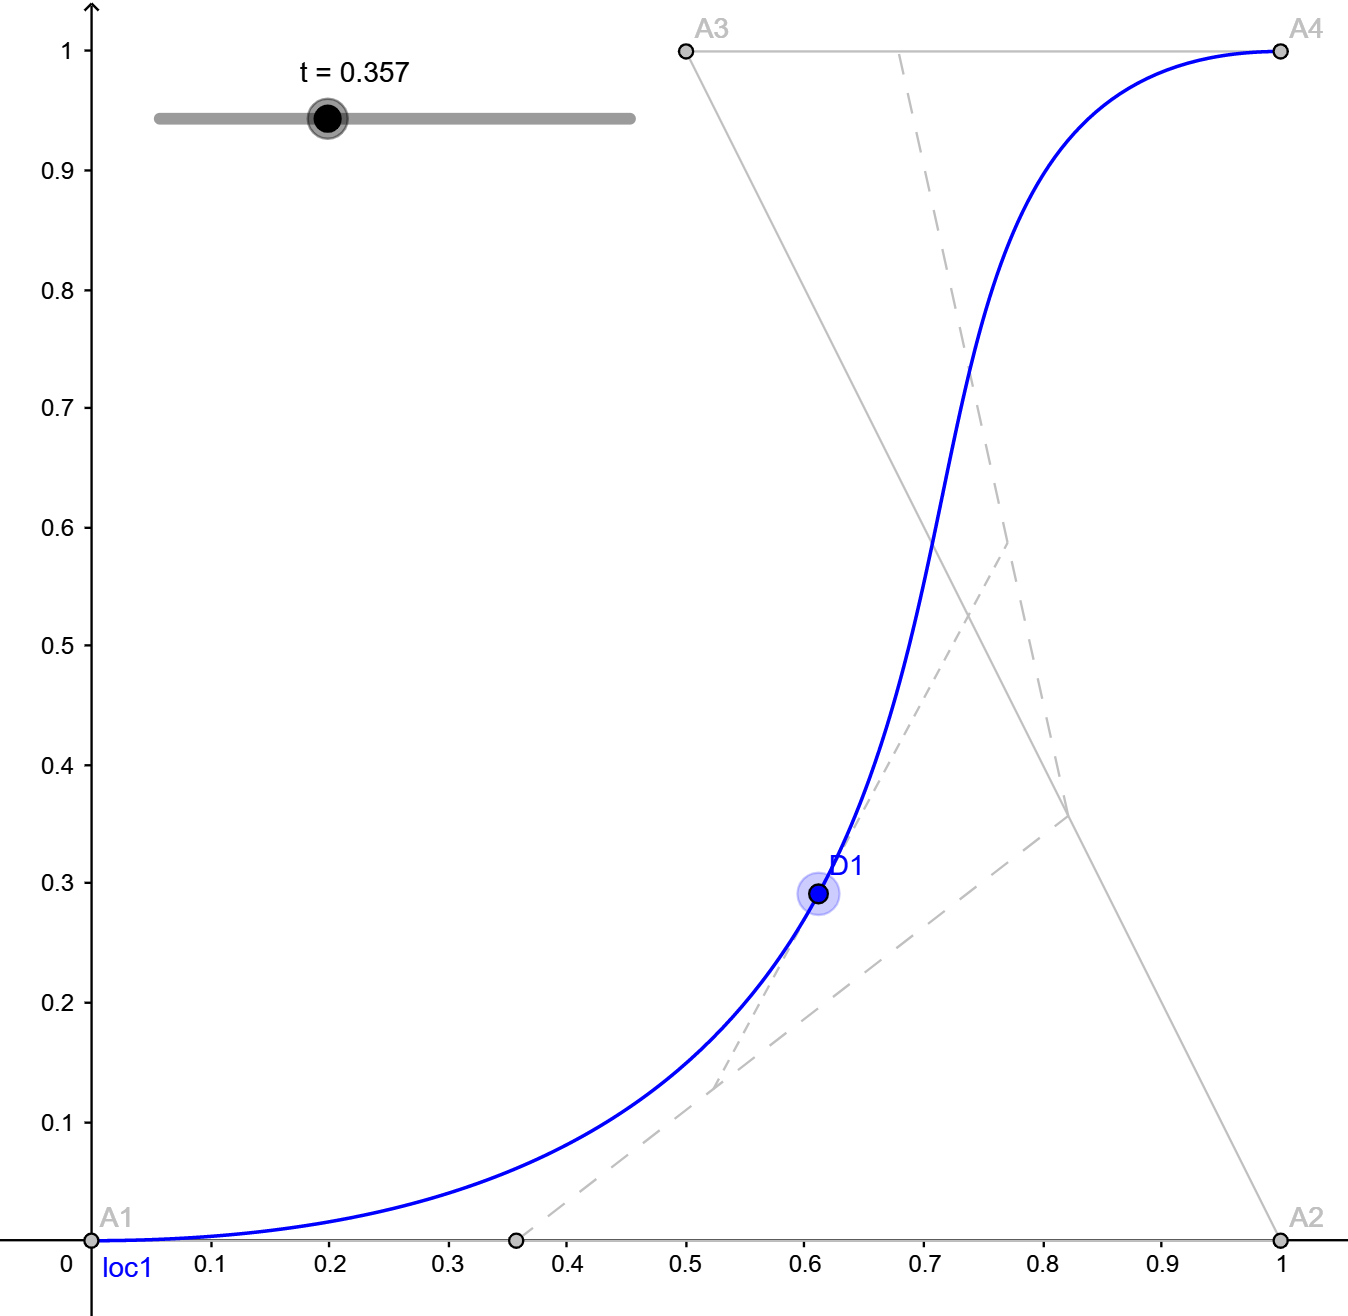
\includegraphics[width=0.4\linewidth]{../common/03_billiard_ai/resources/30_suchbaum_gewichtung_winkelkosten.png}
    \end{center}
    \caption{Gewichtung der Winkelkosten mittels einer Bézier-Kurve.
    Kleine Winkel werden in den Kosten geringer gewichtet, während grosse Winkel eine höhere Gewichtung erhalten.}
    \label{fig:suche_knoten_gewichtung_winkelkosten}
\end{figure}

Das Kriterium der Indirektion über Kugeln wird wiederum über einen maximal möglichen Wert gelöst.
Es wird eine maximale Indirektion $K_{I,max}$ angegeben und die Anzahl der Vorkommnisse ${K_{I,n}}$ wird durch die
Konstante dividiert. Dadurch werden die Kosten erhöht, je grösser der Indirektionsgrad ist.
\begin{align}
    K_{I,krit} = \frac{K_{I,n}}{K_{I,max}}
\end{align}

Das Kriterium der Indirektion über Banden wird ebenso über einen maximal möglichen Wert gelöst.
Es wird eine maximale Indirektion $K_{B,max}$ angegeben und die Anzahl der Vorkomnisse ${K_{B,n}}$ wird durch die
Konstante dividiert. Dadurch werden die Kosten erhöht, je grösser der Indirektionsgrad ist.
\begin{align}
    K_{B,krit} = \frac{K_{B,n}}{K_{B,max}}
\end{align}

Die endgültigen Kosten werden über die Addition aller Kriterien gebildet.
\begin{align}
    K = d_{krit} + \alpha^G_{krit, y} + K_{I,krit} + K_{B,krit}
\end{align}


\newpage
\section{Vergleich Simulation und Realität}\label{kap:vergleich_simulation_und_realitaet}
Um die Realitätsnähe der Simulation zu quantifizieren, wird der Ansatz über die Analyse von Aufnahmen diverser real
durchgeführter Stösse verfolgt.
Dabei ist die Geschwindigkeit, welche die Kugel zu Beginn durch den Queue erfährt, unbekannt.
Diese wird in einem ersten Schritt eruiert.
Bekannt dabei ist die Zeit sowie die Distanz, welche über die Auswahl einzelner Frames berechnet werden.
Die Zeit ergibt sich durch den Abstand zweier Frames.
Bei einem Video mit 30 FPS liegt der Fehler bei $\frac{1}{30} t [s] = 0.03 [s]$.
Die Distanz wird über zwei selektierte Pixelpositionen auf denselben Frames zur Berechnung der Zeit bestimmt.
Diese Positionen werden zu Modellkoordinaten $P_0, P_1$ übersetzt\cite{project2:pixel_to_model_coordinates},
um die Distanz in der Einheit $[mm]$ anzugeben.
Anschliessend kann über die Formel \ref{eq:simvsReal:initialVelocity} die Anfangsgeschwindigkeit berechnet
werden, wobei auch die Gleitreibung $\mu_g$ sowie die Rollreibung $\mu_r$ bekannt sein müssen\footnote{Die Herleitung
erfolgt in Kapitel \ref{anhang:herleitung:initialVelocityWithTime}.}.
\begin{align}
    v_0^2 \cdot \frac{2 \cdot (\mu_g - \mu_r)}{49 \cdot g \cdot \mu_g^2} + v_0 \cdot \frac{t \cdot (2 \cdot \mu_r + 5 \cdot \mu_g)}{7 \cdot \mu_g} - \frac{1}{2} \cdot g \cdot \mu_r \cdot t^2 - s = 0\label{eq:simvsReal:initialVelocity}
\end{align}

Es wird eine quadratische Formel gelöst, welche zwei Resultate $v^1_0, v^2_0$ liefert. Von diesen wird nur die
kleinste positive Lösung $v_0$ in Betracht gezogen.

Sobald $v_0$ bestimmt ist, kann der Geschwindigkeitsvektor $\vec{v_0}$ berechnet werden. Dies geschieht über den Einheitsvektor,
welcher über die beiden Punkte zur Bestimmung der Distanz gegeben ist:
\begin{align}
    \vec{d} &= P_1 - P_0\\
    \hat{d} &= \frac{\vec{d}}{\norm{\vec{d}}}\\
    \vec{v_0} &= v_0 \cdot \hat{d}
\end{align}

Im nächsten Schritt kann die Simulation mit der errechneten Startgeschwindigkeit des Spielballs ausgeführt werden.
Daraus resultiert eine Abfolge von Ereignissen, die in der Simulation gefunden wurden.
Diese werden mit manuell erstellten Ereignissabfolgen abgeglichen, bei welchem alle Positionen der Kugeln und Ereigniszeitpunkte
anhand der Videoaufnahmen bestimmt wurden.
Die Summe der Differenzen zwischen den erwarteten Zeiten und Positionen bilden den Gesamtfehler.

In den Informationen, welche aus den Videos extrahiert wurden, ist ein gewisser Fehler enthalten.
Zudem wird davon ausgegangen, dass bei den durchgeführten Stössen kein Spin enthalten ist, obwohl das gut möglich ist.
Damit können die entstehenden Differenzen nicht exakt verglichen werden.

\newpage
\subsection{Vergleich Stoss ohne Banden}
In diesem Abschnitt werden einige real durchgeführte und aufgezeichnete Stösse vorgestellt und die extrahierten Informationen mit
dem Resultat der Simulation verglichen.
Diese Stösse beinhalten keine Bandeninteraktionen, sondern lediglich die Interaktionen zwischen Kugeln.

\subsubsection{Stoss 1}
Im Ersten Stoss wird eine rote Kugel auf direktem Wege mit hoher Geschwindigkeit in das zentrale untere Loch gespielt.
Wegen der hohen Geschwindigkeit gleitet die weisse Kugel höchstwahrscheinlich noch bei der Kollision mit der roten Kugel.
In Abbildung \ref{fig:simulation_vs_reality_1_0008_0011} sind einige Bilder aus dem aufgezeichneten Video und ein Bild
der Simulation aufgeführt.

Für den Vergleich wurden einige Kennzahlen aus dem Video extrahiert, dies beinhaltet die Positionen der Kugeln
in Modellkoordinaten zu verschiedenen Ereignissen, sowie der Zeitpunkt (gemessen am Startzeitpunkt des Stosses) dieser Ereignisse.
In Tabelle \ref{tab:simulation_vs_reality_1_0008_0011} sind diese Kennzahlen im Vergleich und deren Differenzen aufgeführt.
Damit ist der Fehler der Simulation ersichtlich.
Der Fehler in der Position und dem Zeitpunkt des Stillstands der weissen Kugel ist vorhanden, aber gering.
In der Simulation rollt die weisse Kugel nach der Kollision noch kurz nach rechts-vorne.
Es gilt allerdings zu beachten, dass in den aus dem Video extrahierten Kennzahlen ebenfalls ein
gewisser Fehler enthalten ist, der den Vergleich schwierig macht.

\begin{figure}[h!]
    \centering
    \begin{subfigure}[t]{0.2\textwidth}
        \centering
        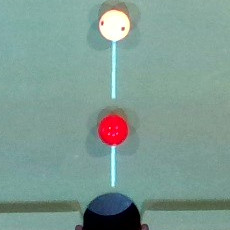
\includegraphics[width=1.0\linewidth]{../common/04_results/resources/simulation_vs_reality/simulation_vs_reality_1_0008_0011_situation_cut.jpg}
        \caption{Startsituation vor dem Stoss.}
        \label{fig:simulation_vs_reality_1_0008_0011_situation}
    \end{subfigure}
    \hfill
    \begin{subfigure}[t]{0.2\textwidth}
        \centering
        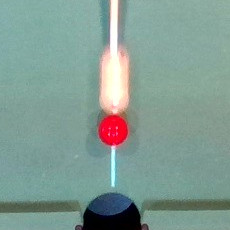
\includegraphics[width=1.0\linewidth]{../common/04_results/resources/simulation_vs_reality/simulation_vs_reality_1_0008_0011_collision_cut.jpg}
        \caption{Kollisionszeitpunkt, der \emph{motion blur} entsteht aufgrund der Geschwindigkeit der weissen Kugel.}
        \label{fig:simulation_vs_reality_1_0008_0011_collision}
    \end{subfigure}
    \hfill
    \begin{subfigure}[t]{0.2\textwidth}
        \centering
        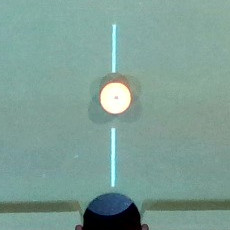
\includegraphics[width=1.0\linewidth]{../common/04_results/resources/simulation_vs_reality/simulation_vs_reality_1_0008_0011_end_cut.jpg}
        \caption{Endzustand nach dem Stoss.}
        \label{fig:simulation_vs_reality_1_0008_0011_end}
    \end{subfigure}
    \hfill
    \begin{subfigure}[t]{0.2\textwidth}
        \centering
        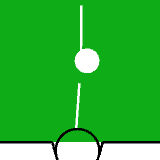
\includegraphics[width=1.0\linewidth]{../common/04_results/resources/simulation_vs_reality/simulation_vs_reality_1_0008_0011_simulation_cut.png}
        \caption{Endzustand nach dem Stoss gemäss Simulation.}
        \label{fig:simulation_vs_reality_1_0008_0011_simulation}
    \end{subfigure}
    \caption{
        Ablauf von Stoss 1: Die weisse Kugel wird mit hoher Geschwindigkeit angestossen, trifft die rote Kugel und locht diese ein.
        Die weisse Kugel steht sofort nach der Kollision still.
    }
    \label{fig:simulation_vs_reality_1_0008_0011}
\end{figure}

\begin{table}[ht]
    \rowcolors{1}{\seccolor!10}{\seccolor!10} % Rows with 10% of secondary color
    \begin{tabular}{ lrrr }
        \rowcolor{\seccolor!50}
        Kennzahl & Wert gemäss Video & Wert gemäss Simulation & Differenz \\
        Start: Position weisse Kugel & (8.38658, -159.215) & - & -\\
        Start: Position rote Kugel & (4.24078, -336.939) & - & -\\
        Kollision: Position weisse Kugel & (7.84763, -284.44) & (7.84627, -284.756) & 0.315677mm\\
        Einlochen: Zeitpunkt rote Kugel wird eingelocht & 0.133333s & 0.172932s & +0.039598s\\
        Stillstand: Position weisse Kugel & (9.53746, -284.455) & (21.7098, -285.714) & 12.237230mm\\
        Stillstand: Zeitpunkt & 0.2s & 0.530894s & +0.330895\\
    \end{tabular}
    \caption{Vergleich Video und Simulation für Stoss 1}
    \label{tab:simulation_vs_reality_1_0008_0011}
\end{table}

\subsubsection{Stoss 2}
Stoss 2 bildet dieselbe Ausgangssituation wie Stoss 1, allerdings wird die weisse Kugel mit einer tieferen Geschwindigkeit angespielt.
In Abbildung \ref{fig:simulation_vs_reality_1_0028_0032} ist der Ablauf des Stosses sowie der Endzustand der Simulation abgebildet.
Aus Tabelle \ref{tab:simulation_vs_reality_1_0028_0032} ist der Positionsfehler der weissen Kugel beim Stillstand auffallend.
Die Simulation hat die weisse Kugel nach der Kollision zu wenig weit rollen lassen.
Das kann auf die Reibungskoeffizienten, den Energieverlust bei Kugelkollision oder die eingegebene Startgeschwindigkeit zurückzuführen sein.

\begin{figure}[h!]
    \centering
    \begin{subfigure}[t]{0.2\textwidth}
        \centering
        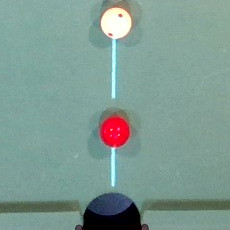
\includegraphics[width=1.0\linewidth]{../common/04_results/resources/simulation_vs_reality/simulation_vs_reality_1_0028_0032_situation_cut.jpg}
        \caption{Startsituation vor dem Stoss.}
        \label{fig:simulation_vs_reality_1_0028_0032_situation}
    \end{subfigure}
    \hfill
    \begin{subfigure}[t]{0.2\textwidth}
        \centering
        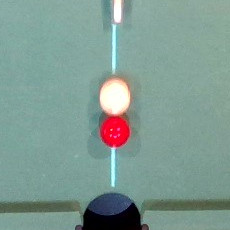
\includegraphics[width=1.0\linewidth]{../common/04_results/resources/simulation_vs_reality/simulation_vs_reality_1_0028_0032_collision_cut.jpg}
        \caption{Kollisionszeitpunkt.}
        \label{fig:simulation_vs_reality_1_0028_0032_collision}
    \end{subfigure}
    \hfill
    \begin{subfigure}[t]{0.2\textwidth}
        \centering
        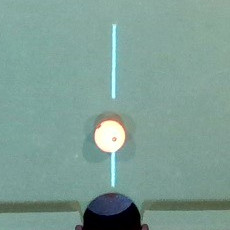
\includegraphics[width=1.0\linewidth]{../common/04_results/resources/simulation_vs_reality/simulation_vs_reality_1_0028_0032_end_cut.jpg}
        \caption{Endzustand nach dem Stoss.}
        \label{fig:simulation_vs_reality_1_0028_0032_end}
    \end{subfigure}
    \hfill
    \begin{subfigure}[t]{0.2\textwidth}
        \centering
        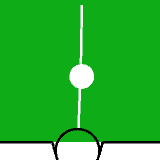
\includegraphics[width=1.0\linewidth]{../common/04_results/resources/simulation_vs_reality/simulation_vs_reality_1_0028_0032_simulation_cut.png}
        \caption{Endzustand nach dem Stoss gemäss Simulation.}
        \label{fig:simulation_vs_reality_1_0028_0032_simulation}
    \end{subfigure}
    \caption{
        Ablauf von Stoss 2: Die weisse Kugel wird mit tiefer Geschwindigkeit angestossen, trifft die rote Kugel und locht diese ein.
        Die weisse Kugel rollt nach der Kollision noch kurz nach vorne.
    }
    \label{fig:simulation_vs_reality_1_0028_0032}
\end{figure}

\begin{table}[ht]
    \rowcolors{1}{\seccolor!10}{\seccolor!10} % Rows with 10% of secondary color
    \begin{tabular}{ lrrr }
        \rowcolor{\seccolor!50}
        Kennzahl & Wert gemäss Video & Wert gemäss Simulation & Differenz \\
        Start: Position weisse Kugel & (9.99188, -157.766) & - & -\\
        Start: Position rote Kugel & (5.8054, -342.29) & - & -\\
        Kollision: Position weisse Kugel & (7.72594, -289.771) & (7.72172, -290.017) & 0.245703mm\\
        Einlochen: Zeitpunkt rote Kugel wird eingelocht & 0.7s & 0.687573s & -0.012427s\\
        Stillstand: Position weisse Kugel & (-2.68527, -350.685) & (9.62618, -321.478) & 31.695890mm\\
        Stillstand: Zeitpunkt & 1.3s & 0.972639s & -0.327361s\\
    \end{tabular}
    \caption{Vergleich Video und Simulation für Stoss 2}
    \label{tab:simulation_vs_reality_1_0028_0032}
\end{table}

\subsubsection{Stoss 3}
In dieser Situation wird eine rote Kugel in einem Winkel von der weissen Kugel mit einer kleinen Geschwindigkeit angespielt.
Die beiden Kugeln rollen nach der Kollision eine kurze Zeit weiter und kommen dann zum Stillstand.
Der Ablauf ist in Abbildung \ref{fig:video_12_0205_0208} und der Vergleich in Tabelle \ref{tab:video_12_0205_0208} dargestellt.
Zusätzlich zu den Positionen und Zeiten der Ereignisse sind zusätzlich die Richtungen, in welche die Kugeln nach der Kollision
rollen, enthalten.
Der Positionsfehler beträgt beim Stillstand ca. 2cm und die Richtung unterscheidet sich bei der roten Kugel um $7^{\circ}$.

\begin{figure}[h!]
    \centering
    \begin{subfigure}[t]{0.2\textwidth}
        \centering
        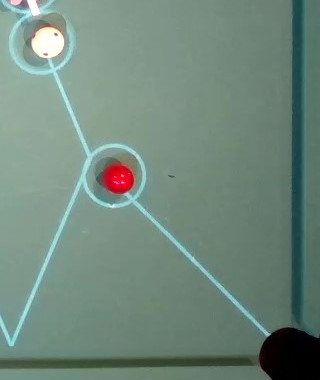
\includegraphics[width=1.0\linewidth]{../common/04_results/resources/simulation_vs_reality/video_12_0205_0208_situation_cut.jpg}
        \caption{Startsituation vor dem Stoss.}
        \label{fig:video_12_0205_0208_situation}
    \end{subfigure}
    \hfill
    \begin{subfigure}[t]{0.2\textwidth}
        \centering
        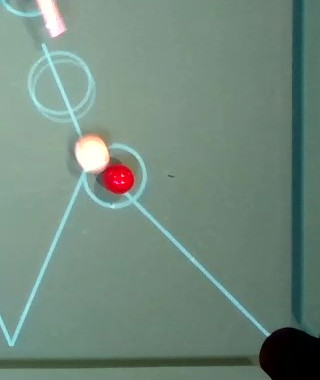
\includegraphics[width=1.0\linewidth]{../common/04_results/resources/simulation_vs_reality/video_12_0205_0208_collision_cut.jpg}
        \caption{Kollisionszeitpunkt.}
        \label{fig:video_12_0205_0208_collision}
    \end{subfigure}
    \hfill
    \begin{subfigure}[t]{0.2\textwidth}
        \centering
        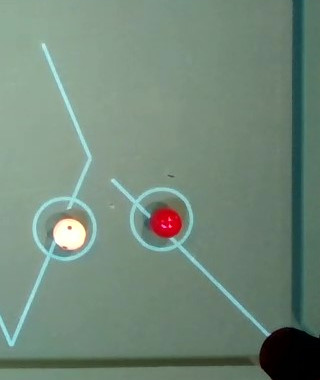
\includegraphics[width=1.0\linewidth]{../common/04_results/resources/simulation_vs_reality/video_12_0205_0208_end_cut.jpg}
        \caption{Endzustand nach dem Stoss.}
        \label{fig:video_12_0205_0208_end}
    \end{subfigure}
    \hfill
    \begin{subfigure}[t]{0.2\textwidth}
        \centering
        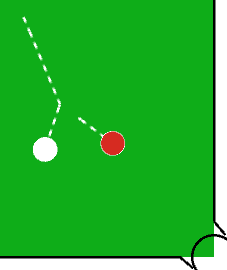
\includegraphics[width=1.0\linewidth]{../common/04_results/resources/simulation_vs_reality/video_12_0205_0208_simulation_cut.png}
        \caption{Endzustand nach dem Stoss gemäss Simulation.}
        \label{fig:video_12_0205_0208_simulation}
    \end{subfigure}
    \caption{
        Ablauf von Stoss 3: Die weisse Kugel wird mit tiefer Geschwindigkeit angestossen und trifft die rote Kugel.
        Beide Kugeln rollen nach der Kollision weiter und bleiben nach kurzer Zeit stehen.
    }
    \label{fig:video_12_0205_0208}
\end{figure}

\begin{table}[ht]
    \rowcolors{1}{\seccolor!10}{\seccolor!10} % Rows with 10% of secondary color
    \begin{tabular}{ lrrr }
        \rowcolor{\seccolor!50}
        Kennzahl & Wert gemäss Video & Wert gemäss Simulation & Differenz \\
        Start: Position weisse Kugel & (504.88, 77.68) & - & -\\
        Start: Position rote Kugel & (630.137, -152.789) & - & -\\
        Kollision: Position weisse Kugel & (585.423, -114.962) & (588.18, -121.556) & 7.146715mm\\
        Rollen nach Kollision: Richtung weisse Kugel & (-0.288612, -0.957446) & (-0.309209, -0.950994) & 1.236697$^{\circ}$ \\
        Rollen nach Kollision: Richtung rote Kugel & (0.715309, -0.698809) & (0.802148, -0.597126) & 7.667131$^{\circ}$ \\
        Stillstand: Position weisse Kugel & (545.906, -246.056) & (554.434, -225.344) & 22.398825mm\\
        Stillstand: Zeitpunkt weisse Kugel & 2.233333s & 1.909805s & -0.323528s\\
        Stillstand: Position rote Kugel & (709.469, -230.291) & (709.088, -211.561) & 18.734226mm\\
        Stillstand: Zeitpunkt rote Kugel & 1.933333s & 1.840109s & -0.093224s\\
    \end{tabular}
    \caption{Vergleich Video und Simulation für Stoss 3}
    \label{tab:video_12_0205_0208}
\end{table}

\newpage
\subsubsection{Stoss 4}
Mit Stoss 4 wird die rote Kugel in gerader Linie von der weissen Kugel mit mittlerer Geschwindigkeit eingelocht,
siehe Abbildung \ref{fig:video_13_0030_0034}.
Aus Tabelle \ref{tab:video_13_0030_0034} sind kleine zeitliche Differenzen ersichtlich und
ein Positionsfehler beim Stillstand der weissen Kugel von 2,6cm.

\begin{figure}[h!]
    \centering
    \begin{subfigure}[t]{0.2\textwidth}
        \centering
        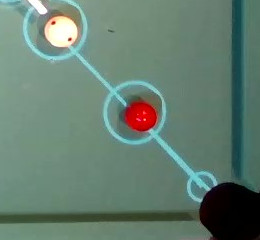
\includegraphics[width=1.0\linewidth]{../common/04_results/resources/simulation_vs_reality/video_13_0030_0034_situation_cut.jpg}
        \caption{Startsituation vor dem Stoss.}
        \label{fig:video_13_0030_0034_situation}
    \end{subfigure}
    \hfill
    \begin{subfigure}[t]{0.2\textwidth}
        \centering
        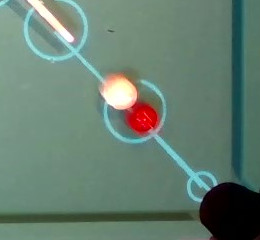
\includegraphics[width=1.0\linewidth]{../common/04_results/resources/simulation_vs_reality/video_13_0030_0034_collision_cut.jpg}
        \caption{Kollisionszeitpunkt.}
        \label{fig:video_13_0030_0034_collision}
    \end{subfigure}
    \hfill
    \begin{subfigure}[t]{0.2\textwidth}
        \centering
        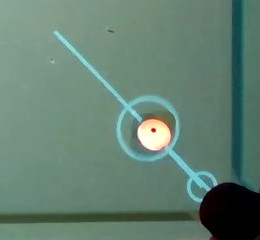
\includegraphics[width=1.0\linewidth]{../common/04_results/resources/simulation_vs_reality/video_13_0030_0034_end_cut.jpg}
        \caption{Endzustand nach dem Stoss.}
        \label{fig:video_13_0030_0034_end}
    \end{subfigure}
    \hfill
    \begin{subfigure}[t]{0.2\textwidth}
        \centering
        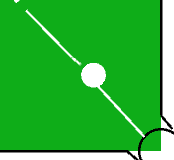
\includegraphics[width=1.0\linewidth]{../common/04_results/resources/simulation_vs_reality/video_13_0030_0034_simulation_cut.png}
        \caption{Endzustand nach dem Stoss gemäss Simulation.}
        \label{fig:video_13_0030_0034_simulation}
    \end{subfigure}
    \caption{
        Ablauf von Stoss 4: Die weisse Kugel wird mit mittlerer Geschwindigkeit angestossen, trifft die rote Kugel und locht diese ein.
        Die weisse Kugel rollt nach der Kollision noch kurz nach vorne.
    }
    \label{fig:video_13_0030_0034}
\end{figure}

\begin{table}[ht]
    \rowcolors{1}{\seccolor!10}{\seccolor!10} % Rows with 10% of secondary color
    \begin{tabular}{ lrrr }
        \rowcolor{\seccolor!50}
        Kennzahl & Wert gemäss Video & Wert gemäss Simulation & Differenz \\
        Start: Position weisse Kugel & (631.828, -149.426) & - & -\\
        Start: Position rote Kugel & (771.566, -295.777) & - & -\\
        Kollision: Position weisse Kugel & (735.251, -256.098) & (736.286, -257.165) & 1.486228mm\\
        Einlochen: Zeitpunkt rote Kugel wird eingelocht & 0.8s & 0.765598s & -0.034402s\\
        Stillstand: Position weisse Kugel & (792.353, -323.378) & (786.198, -297.818) & 26.290272mm\\
        Stillstand: Zeitpunkt & 1.2s & 1.196382s & -0.003618s\\
    \end{tabular}
    \caption{Vergleich Video und Simulation für Stoss 4}
    \label{tab:video_13_0030_0034}
\end{table}

Damit wurden anhand einiger Stösse, welche keine Bandeninteraktion enthalten,
der Vergleich zwischen Simulation und Realität gezogen und quantitativ ausgewertet.
Die Auswertung ist nicht fehlerfrei, ergibt allerdings einen Rahmen, in dem sich die Genauigkeit der Simulation in diesen
Situationen bewegt.

\newpage
\subsection{Vergleich Bandenstoss}\label{kap:vergleich_simulation_realitaet:vergleich_bandenstoss}
Dieses Kapitel widmet sich dem Abgleich des erwarteten Verhaltens bei einer Bandenkollision wie in
Abschnitt \ref{kandidatensuche:bandenkollisionstheorie} beschrieben und dem effektiven Verhalten des verwendeten Tisches.
Es wird in zwei Subkapitel gegliedert, wobei sich das Erste mit der Beschreibung der Realität befasst, das Zweite hingegen
mit der Diskussion der Resultate.

\subsubsection{Bandenkollisionsrealität}
Es folgt die Beschreibung eines experimentellen Vorgehens, um zu prüfen, ob die Banden des verwendeten Billardtisches den
bekannten theoretischen und praktischen Vorgaben entsprechen. Dafür wurden zwei Videos aufgenommen und analysiert,
die einen schwächeren und einen starken Stoss zeigen.
Nach der beschriebenen Theorie müsste der Ausfallswinkel in etwa dem Einfallswinkel entsprechen.
Um einen Anhaltspunkt zu gewinnen, wurde ein Stoss
über eine Bande gesucht. Dadurch werden Linien auf den Tisch projiziert, die die Ausführung des Experiments vereinfachen.
Die angestossene Kugel müsste den visualisierten Linien folgen, sollte die Theorie auf den verwendeten Billardtisch
anwendbar sein.

Beim nachfolgend präsentierten schwachen Stoss in Abbildung \ref{fig:kugelverlauf_nach_bandenkollision_mit_schwachem_stoss_pool} wird erwartet, dass der Ausfallswinkel gemäss dem Prinzip 6.7 aus
Abschnitt \ref{kandidatensuche:bandenkollisionstheorie} grösser ausfällt. Dem ist effektiv so, jedoch ist
der Ausfallswinkel viel zu gross und kommt nicht durch den beschriebenen Topspin zustande, da die Kugel zu Beginn
eigentlich durchaus dem theoretischen Ausfallsweg folgen sollte. In Abbildung \ref{fig:rebound_angle_no_spin_slow_shot} sind
einzelne Frames des Stosses ersichtlich. Bis zum Bandenaufprall folgt die weisse Kugel dem erwarteten Pfad. Bereits nach
dem Bandenaufprall in $f$ kann eine leichte seitliche Verschiebung der Kugel erkannt werden, welche den weiteren Verlauf
stark beeinflusst.

\begin{figure}[h!]
    \centering
    \begin{subfigure}[b]{0.2\textwidth}
        \centering
        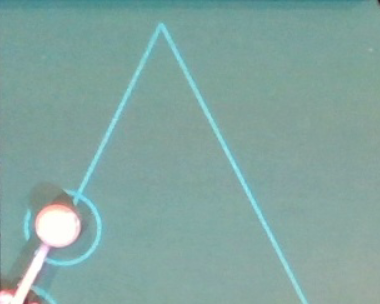
\includegraphics[width=1.0\linewidth]{../common/04_results/resources/simulation/rebound_angle_slow_pool/00_rail_rebound_angle_slow_pool_01.png}
        \caption{Ausfallswinkel bei schwachem Stoss in Pool - 1}
        \label{fig:rebound_angle_slow_pool_1}
    \end{subfigure}
    \hfill
    \begin{subfigure}[b]{0.2\textwidth}
        \centering
        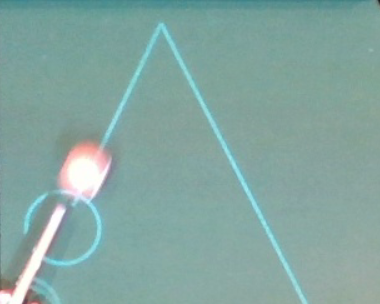
\includegraphics[width=1.0\linewidth]{../common/04_results/resources/simulation/rebound_angle_slow_pool/00_rail_rebound_angle_slow_pool_02.png}
        \caption{Ausfallswinkel bei schwachem Stoss in Pool - 2}
        \label{fig:rebound_angle_slow_pool_2}
    \end{subfigure}
    \hfill
    \begin{subfigure}[b]{0.2\textwidth}
        \centering
        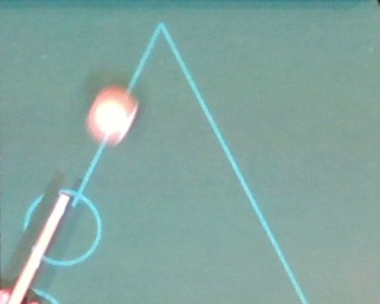
\includegraphics[width=1.0\linewidth]{../common/04_results/resources/simulation/rebound_angle_slow_pool/00_rail_rebound_angle_slow_pool_03.png}
        \caption{Ausfallswinkel bei schwachem Stoss in Pool - 3}
        \label{fig:rebound_angle_slow_pool_3}
    \end{subfigure}
    \hfill
    \begin{subfigure}[b]{0.2\textwidth}
        \centering
        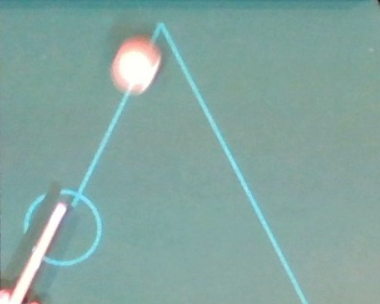
\includegraphics[width=1.0\linewidth]{../common/04_results/resources/simulation/rebound_angle_slow_pool/00_rail_rebound_angle_slow_pool_04.png}
        \caption{Ausfallswinkel bei schwachem Stoss in Pool - 4}
        \label{fig:rebound_angle_slow_pool_4}
    \end{subfigure}
    \hfill
    \begin{subfigure}[b]{0.2\textwidth}
        \centering
        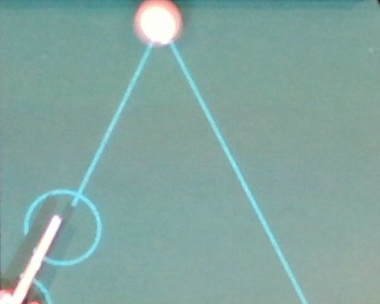
\includegraphics[width=1.0\linewidth]{../common/04_results/resources/simulation/rebound_angle_slow_pool/00_rail_rebound_angle_slow_pool_05.png}
        \caption{Ausfallswinkel bei schwachem Stoss in Pool - 5}
        \label{fig:rebound_angle_slow_pool_5}
    \end{subfigure}
    \hfill
    \begin{subfigure}[b]{0.2\textwidth}
        \centering
        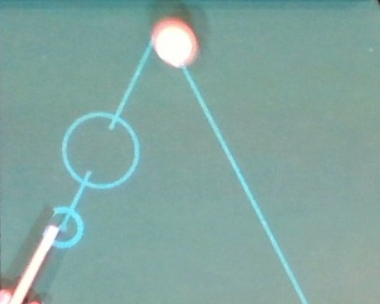
\includegraphics[width=1.0\linewidth]{../common/04_results/resources/simulation/rebound_angle_slow_pool/00_rail_rebound_angle_slow_pool_06.png}
        \caption{Ausfallswinkel bei schwachem Stoss in Pool - 6}
        \label{fig:rebound_angle_slow_pool_6}
    \end{subfigure}
    \hfill
    \begin{subfigure}[b]{0.2\textwidth}
        \centering
        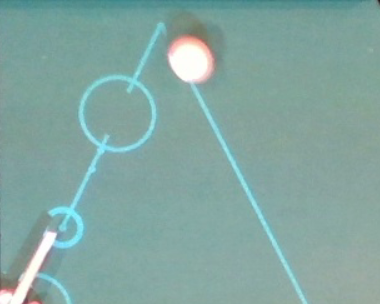
\includegraphics[width=1.0\linewidth]{../common/04_results/resources/simulation/rebound_angle_slow_pool/00_rail_rebound_angle_slow_pool_07.png}
        \caption{Ausfallswinkel bei schwachem Stoss in Pool - 7}
        \label{fig:rebound_angle_slow_pool_7}
    \end{subfigure}
    \hfill
    \begin{subfigure}[b]{0.2\textwidth}
        \centering
        \includegraphics[width=1.0\linewidth]{../common/04_results/resources/simulation/rebound_angle_slow_pool/00_rail_rebound_angle_slow_pool_08.png}
        \caption{Ausfallswinkel bei schwachem Stoss in Pool - 8}
        \label{fig:rebound_angle_slow_pool_8}
    \end{subfigure}
    \hfill
    \begin{subfigure}[b]{0.2\textwidth}
        \centering
        \includegraphics[width=1.0\linewidth]{../common/04_results/resources/simulation/rebound_angle_slow_pool/00_rail_rebound_angle_slow_pool_09.png}
        \caption{Ausfallswinkel bei schwachem Stoss in Pool - 9}
        \label{fig:rebound_angle_slow_pool_9}
    \end{subfigure}
    \hfill
    \begin{subfigure}[b]{0.2\textwidth}
        \centering
        \includegraphics[width=1.0\linewidth]{../common/04_results/resources/simulation/rebound_angle_slow_pool/00_rail_rebound_angle_slow_pool_10.png}
        \caption{Ausfallswinkel bei schwachem Stoss in Pool - 10}
        \label{fig:rebound_angle_slow_pool_10}
    \end{subfigure}
    \hfill
    \begin{subfigure}[b]{0.2\textwidth}
        \centering
        \includegraphics[width=1.0\linewidth]{../common/04_results/resources/simulation/rebound_angle_slow_pool/00_rail_rebound_angle_slow_pool_11.png}
        \caption{Ausfallswinkel bei schwachem Stoss in Pool - 11}
        \label{fig:rebound_angle_slow_pool_11}
    \end{subfigure}
    \hfill
    \begin{subfigure}[b]{0.2\textwidth}
        \centering
        \includegraphics[width=1.0\linewidth]{../common/04_results/resources/simulation/rebound_angle_slow_pool/00_rail_rebound_angle_slow_pool_12.png}
        \caption{Ausfallswinkel bei schwachem Stoss in Pool - 12}
        \label{fig:rebound_angle_slow_pool_12}
    \end{subfigure}
    \caption{Kugelverlauf nach Bandenkollision mit schwachem Stoss - Pool}
    \label{fig:kugelverlauf_nach_bandenkollision_mit_schwachem_stoss_pool}
\end{figure}

Der starke Stoss wird in Abbildung \ref{fig:kugelverlauf_nach_bandenkollision_mit_starkem_stoss_pool} thematisiert.
Erwartet wird nach dem Prinzip 6.6 aus Kapitel \ref{kandidatensuche:bandenkollisionstheorie} ein kleinerer Ausfallswinkel als der Eingezeichnete.
Effektiv resultiert aber auch in diesem Fall wie im vorherig beschriebenen Fall ein grösserer Ausfallswinkel.
Nach dem Bandenaufprall in $f$ kann ebenso wieder eine leichte Versetzung der Kugel ausgemacht werden, die einen
grossen Einfluss hat.

\begin{figure}[h!]
    \centering
    \begin{subfigure}[b]{0.2\textwidth}
        \centering
        \includegraphics[width=1.0\linewidth]{../common/04_results/resources/simulation/rebound_angle_fast_pool/00_rail_rebound_angle_fast_pool_01.png}
        \caption{Ausfallswinkel bei starkem Stoss in Pool - 1}
        \label{fig:rebound_angle_fast_pool_1}
    \end{subfigure}
    \hfill
    \begin{subfigure}[b]{0.2\textwidth}
        \centering
        \includegraphics[width=1.0\linewidth]{../common/04_results/resources/simulation/rebound_angle_fast_pool/00_rail_rebound_angle_fast_pool_02.png}
        \caption{Ausfallswinkel bei starkem Stoss in Pool - 2}
        \label{fig:rebound_angle_fast_pool_2}
    \end{subfigure}
    \hfill
    \begin{subfigure}[b]{0.2\textwidth}
        \centering
        \includegraphics[width=1.0\linewidth]{../common/04_results/resources/simulation/rebound_angle_fast_pool/00_rail_rebound_angle_fast_pool_03.png}
        \caption{Ausfallswinkel bei starkem Stoss in Pool - 3}
        \label{fig:rebound_angle_fast_pool_3}
    \end{subfigure}
    \hfill
    \begin{subfigure}[b]{0.2\textwidth}
        \centering
        \includegraphics[width=1.0\linewidth]{../common/04_results/resources/simulation/rebound_angle_fast_pool/00_rail_rebound_angle_fast_pool_04.png}
        \caption{Ausfallswinkel bei starkem Stoss in Pool - 4}
        \label{fig:rebound_angle_fast_pool_4}
    \end{subfigure}
    \hfill
    \begin{subfigure}[b]{0.2\textwidth}
        \centering
        \includegraphics[width=1.0\linewidth]{../common/04_results/resources/simulation/rebound_angle_fast_pool/00_rail_rebound_angle_fast_pool_05.png}
        \caption{Ausfallswinkel bei starkem Stoss in Pool - 5}
        \label{fig:rebound_angle_fast_pool_5}
    \end{subfigure}
    \hfill
    \begin{subfigure}[b]{0.2\textwidth}
        \centering
        \includegraphics[width=1.0\linewidth]{../common/04_results/resources/simulation/rebound_angle_fast_pool/00_rail_rebound_angle_fast_pool_06.png}
        \caption{Ausfallswinkel bei starkem Stoss in Pool - 6}
        \label{fig:rebound_angle_fast_pool_6}
    \end{subfigure}
    \hfill
    \begin{subfigure}[b]{0.2\textwidth}
        \centering
        \includegraphics[width=1.0\linewidth]{../common/04_results/resources/simulation/rebound_angle_fast_pool/00_rail_rebound_angle_fast_pool_07.png}
        \caption{Ausfallswinkel bei starkem Stoss in Pool - 7}
        \label{fig:rebound_angle_fast_pool_7}
    \end{subfigure}
    \hfill
    \begin{subfigure}[b]{0.2\textwidth}
        \centering
        \includegraphics[width=1.0\linewidth]{../common/04_results/resources/simulation/rebound_angle_fast_pool/00_rail_rebound_angle_fast_pool_08.png}
        \caption{Ausfallswinkel bei starkem Stoss in Pool - 8}
        \label{fig:rebound_angle_fast_pool_8}
    \end{subfigure}
    \hfill
    \begin{subfigure}[b]{0.2\textwidth}
        \centering
        \includegraphics[width=1.0\linewidth]{../common/04_results/resources/simulation/rebound_angle_fast_pool/00_rail_rebound_angle_fast_pool_09.png}
        \caption{Ausfallswinkel bei starkem Stoss in Pool - 9}
        \label{fig:rebound_angle_fast_pool_9}
    \end{subfigure}
    \hfill
    \begin{subfigure}[b]{0.2\textwidth}
        \centering
        \includegraphics[width=1.0\linewidth]{../common/04_results/resources/simulation/rebound_angle_fast_pool/00_rail_rebound_angle_fast_pool_10.png}
        \caption{Ausfallswinkel bei starkem Stoss in Pool - 10}
        \label{fig:rebound_angle_fast_pool_10}
    \end{subfigure}
    \hfill
    \begin{subfigure}[b]{0.2\textwidth}
        \centering
        \includegraphics[width=1.0\linewidth]{../common/04_results/resources/simulation/rebound_angle_fast_pool/00_rail_rebound_angle_fast_pool_11.png}
        \caption{Ausfallswinkel bei starkem Stoss in Pool - 11}
        \label{fig:rebound_angle_fast_pool_11}
    \end{subfigure}
    \hfill
    \begin{subfigure}[b]{0.2\textwidth}
        \centering
        \includegraphics[width=1.0\linewidth]{../common/04_results/resources/simulation/rebound_angle_fast_pool/00_rail_rebound_angle_fast_pool_12.png}
        \caption{Ausfallswinkel bei starkem Stoss in Pool - 12}
        \label{fig:rebound_angle_fast_pool_12}
    \end{subfigure}
    \caption{Kugelverlauf nach Bandenkollision mit starkem Stoss - Pool}
    \label{fig:kugelverlauf_nach_bandenkollision_mit_starkem_stoss_pool}
\end{figure}

\newpage
Weiterhin werden anstelle der grösseren Pool-Kugeln kleinere Snooker-Kugeln verwendet. Dies kann ebenfalls einen
Einfluss auf das Zusammenspiel mit der Bande haben. Daher wurden dieselben Experimente, wie sie in diesem Kapitel vorgängig beschrieben
wurden, ebenfalls für Snooker-Kugeln durchgeführt, was den Abbildungen \ref{fig:kugelverlauf_nach_bandenkollision_mit_schwachem_stoss_snooker}
und \ref{fig:kugelverlauf_nach_bandenkollision_mit_starkem_stoss_snooker} zu entnehmen ist.
Das Verhalten ist im Wesentlichen dasselbe, der Ausfallswinkel ist in beiden Fällen viel zu gross.

\begin{figure}[h!]
    \centering
    \begin{subfigure}[b]{0.2\textwidth}
        \centering
        \includegraphics[width=1.0\linewidth]{../common/04_results/resources/simulation/rebound_angle_slow_snooker/00_rail_rebound_angle_slow_snooker_01.png}
        \caption{Ausfallswinkel bei schwachem Stoss in Snooker - 1}
        \label{fig:rebound_angle_slow_snooker_1}
    \end{subfigure}
    \hfill
    \begin{subfigure}[b]{0.2\textwidth}
        \centering
        \includegraphics[width=1.0\linewidth]{../common/04_results/resources/simulation/rebound_angle_slow_snooker/00_rail_rebound_angle_slow_snooker_02.png}
        \caption{Ausfallswinkel bei schwachem Stoss in Snooker - 2}
        \label{fig:rebound_angle_slow_snooker_2}
    \end{subfigure}
    \hfill
    \begin{subfigure}[b]{0.2\textwidth}
        \centering
        \includegraphics[width=1.0\linewidth]{../common/04_results/resources/simulation/rebound_angle_slow_snooker/00_rail_rebound_angle_slow_snooker_03.png}
        \caption{Ausfallswinkel bei schwachem Stoss in Snooker - 3}
        \label{fig:rebound_angle_slow_snooker_3}
    \end{subfigure}
    \hfill
    \begin{subfigure}[b]{0.2\textwidth}
        \centering
        \includegraphics[width=1.0\linewidth]{../common/04_results/resources/simulation/rebound_angle_slow_snooker/00_rail_rebound_angle_slow_snooker_04.png}
        \caption{Ausfallswinkel bei schwachem Stoss in Snooker - 4}
        \label{fig:rebound_angle_slow_snooker_4}
    \end{subfigure}
    \hfill
    \begin{subfigure}[b]{0.2\textwidth}
        \centering
        \includegraphics[width=1.0\linewidth]{../common/04_results/resources/simulation/rebound_angle_slow_snooker/00_rail_rebound_angle_slow_snooker_05.png}
        \caption{Ausfallswinkel bei schwachem Stoss in Snooker - 5}
        \label{fig:rebound_angle_slow_snooker_5}
    \end{subfigure}
    \hfill
    \begin{subfigure}[b]{0.2\textwidth}
        \centering
        \includegraphics[width=1.0\linewidth]{../common/04_results/resources/simulation/rebound_angle_slow_snooker/00_rail_rebound_angle_slow_snooker_06.png}
        \caption{Ausfallswinkel bei schwachem Stoss in Snooker - 6}
        \label{fig:rebound_angle_slow_snooker_6}
    \end{subfigure}
    \hfill
    \begin{subfigure}[b]{0.2\textwidth}
        \centering
        \includegraphics[width=1.0\linewidth]{../common/04_results/resources/simulation/rebound_angle_slow_snooker/00_rail_rebound_angle_slow_snooker_07.png}
        \caption{Ausfallswinkel bei schwachem Stoss in Snooker - 7}
        \label{fig:rebound_angle_slow_snooker_7}
    \end{subfigure}
    \hfill
    \begin{subfigure}[b]{0.2\textwidth}
        \centering
        \includegraphics[width=1.0\linewidth]{../common/04_results/resources/simulation/rebound_angle_slow_snooker/00_rail_rebound_angle_slow_snooker_08.png}
        \caption{Ausfallswinkel bei schwachem Stoss in Snooker - 8}
        \label{fig:rebound_angle_slow_snooker_8}
    \end{subfigure}
    \hfill
    \begin{subfigure}[b]{0.2\textwidth}
        \centering
        \includegraphics[width=1.0\linewidth]{../common/04_results/resources/simulation/rebound_angle_slow_snooker/00_rail_rebound_angle_slow_snooker_09.png}
        \caption{Ausfallswinkel bei schwachem Stoss in Snooker - 9}
        \label{fig:rebound_angle_slow_snooker_9}
    \end{subfigure}
    \hfill
    \begin{subfigure}[b]{0.2\textwidth}
        \centering
        \includegraphics[width=1.0\linewidth]{../common/04_results/resources/simulation/rebound_angle_slow_snooker/00_rail_rebound_angle_slow_snooker_10.png}
        \caption{Ausfallswinkel bei schwachem Stoss in Snooker - 10}
        \label{fig:rebound_angle_slow_snooker_10}
    \end{subfigure}
    \hfill
    \begin{subfigure}[b]{0.2\textwidth}
        \centering
        \includegraphics[width=1.0\linewidth]{../common/04_results/resources/simulation/rebound_angle_slow_snooker/00_rail_rebound_angle_slow_snooker_11.png}
        \caption{Ausfallswinkel bei schwachem Stoss in Snooker - 11}
        \label{fig:rebound_angle_slow_snooker_11}
    \end{subfigure}
    \hfill
    \begin{subfigure}[b]{0.2\textwidth}
        \centering
        \includegraphics[width=1.0\linewidth]{../common/04_results/resources/simulation/rebound_angle_slow_snooker/00_rail_rebound_angle_slow_snooker_12.png}
        \caption{Ausfallswinkel bei schwachem Stoss in Snooker - 12}
        \label{fig:rebound_angle_slow_snooker_12}
    \end{subfigure}
    \caption{Kugelverlauf nach Bandenkollision mit schwachem Stoss - Snooker}
    \label{fig:kugelverlauf_nach_bandenkollision_mit_schwachem_stoss_snooker}
\end{figure}

\begin{figure}[h!]
    \centering
    \begin{subfigure}[t]{0.2\textwidth}
        \centering
        \includegraphics[width=1.0\linewidth]{../common/04_results/resources/simulation/rebound_angle_fast_snooker/00_rail_rebound_angle_fast_snooker_01.png}
        \caption{Ausfallswinkel bei starkem Stoss in Snooker - 1}
        \label{fig:rebound_angle_fast_snooker_1}
    \end{subfigure}
    \hfill
    \begin{subfigure}[t]{0.2\textwidth}
        \centering
        \includegraphics[width=1.0\linewidth]{../common/04_results/resources/simulation/rebound_angle_fast_snooker/00_rail_rebound_angle_fast_snooker_02.png}
        \caption{Ausfallswinkel bei starkem Stoss in Snooker - 2}
        \label{fig:rebound_angle_fast_snooker_2}
    \end{subfigure}
    \hfill
    \begin{subfigure}[t]{0.2\textwidth}
        \centering
        \includegraphics[width=1.0\linewidth]{../common/04_results/resources/simulation/rebound_angle_fast_snooker/00_rail_rebound_angle_fast_snooker_03.png}
        \caption{Ausfallswinkel bei starkem Stoss in Snooker - 3}
        \label{fig:rebound_angle_fast_snooker_3}
    \end{subfigure}
    \hfill
    \begin{subfigure}[t]{0.2\textwidth}
        \centering
        \includegraphics[width=1.0\linewidth]{../common/04_results/resources/simulation/rebound_angle_fast_snooker/00_rail_rebound_angle_fast_snooker_04.png}
        \caption{Ausfallswinkel bei starkem Stoss in Snooker - 4}
        \label{fig:rebound_angle_fast_snooker_4}
    \end{subfigure}
    \hfill
    \begin{subfigure}[t]{0.2\textwidth}
        \centering
        \includegraphics[width=1.0\linewidth]{../common/04_results/resources/simulation/rebound_angle_fast_snooker/00_rail_rebound_angle_fast_snooker_05.png}
        \caption{Ausfallswinkel bei starkem Stoss in Snooker - 5}
        \label{fig:rebound_angle_fast_snooker_5}
    \end{subfigure}
    \hfill
    \begin{subfigure}[t]{0.2\textwidth}
        \centering
        \includegraphics[width=1.0\linewidth]{../common/04_results/resources/simulation/rebound_angle_fast_snooker/00_rail_rebound_angle_fast_snooker_06.png}
        \caption{Ausfallswinkel bei starkem Stoss in Snooker - 6}
        \label{fig:rebound_angle_fast_snooker_6}
    \end{subfigure}
    \hfill
    \begin{subfigure}[t]{0.2\textwidth}
        \centering
        \includegraphics[width=1.0\linewidth]{../common/04_results/resources/simulation/rebound_angle_fast_snooker/00_rail_rebound_angle_fast_snooker_07.png}
        \caption{Ausfallswinkel bei starkem Stoss in Snooker - 7}
        \label{fig:rebound_angle_fast_snooker_7}
    \end{subfigure}
    \hfill
    \begin{subfigure}[t]{0.2\textwidth}
        \centering
        \includegraphics[width=1.0\linewidth]{../common/04_results/resources/simulation/rebound_angle_fast_snooker/00_rail_rebound_angle_fast_snooker_08.png}
        \caption{Ausfallswinkel bei starkem Stoss in Snooker - 8}
        \label{fig:rebound_angle_fast_snooker_8}
    \end{subfigure}
    \hfill
    \begin{subfigure}[t]{0.2\textwidth}
        \centering
        \includegraphics[width=1.0\linewidth]{../common/04_results/resources/simulation/rebound_angle_fast_snooker/00_rail_rebound_angle_fast_snooker_09.png}
        \caption{Ausfallswinkel bei starkem Stoss in Snooker - 9}
        \label{fig:rebound_angle_fast_snooker_9}
    \end{subfigure}
    \hfill
    \begin{subfigure}[t]{0.2\textwidth}
        \centering
        \includegraphics[width=1.0\linewidth]{../common/04_results/resources/simulation/rebound_angle_fast_snooker/00_rail_rebound_angle_fast_snooker_10.png}
        \caption{Ausfallswinkel bei starkem Stoss in Snooker - 10}
        \label{fig:rebound_angle_fast_snooker_10}
    \end{subfigure}
    \hfill
    \begin{subfigure}[t]{0.2\textwidth}
        \centering
        \includegraphics[width=1.0\linewidth]{../common/04_results/resources/simulation/rebound_angle_fast_snooker/00_rail_rebound_angle_fast_snooker_11.png}
        \caption{Ausfallswinkel bei starkem Stoss in Snooker - 11}
        \label{fig:rebound_angle_fast_snooker_11}
    \end{subfigure}
    \hfill
    \begin{subfigure}[t]{0.2\textwidth}
        \centering
        \includegraphics[width=1.0\linewidth]{../common/04_results/resources/simulation/rebound_angle_fast_snooker/00_rail_rebound_angle_fast_snooker_12.png}
        \caption{Ausfallswinkel bei starkem Stoss in Snooker - 12}
        \label{fig:rebound_angle_fast_snooker_12}
    \end{subfigure}
    \caption{Kugelverlauf nach Bandenkollision mit starkem Stoss - Snooker}
    \label{fig:kugelverlauf_nach_bandenkollision_mit_starkem_stoss_snooker}
\end{figure}

\newpage
An dieser Stelle kann festgehalten werden, dass die Bande des Billardtisches nicht die erwarteten Eigenschaften
aufweist, was wahrscheinlich daran liegt, dass es sich um ein günstig erhältliches Produkt mit entsprechender Qualität handelt.
Anzumerken ist, dass während dem Spielen aufgefallen ist, dass das rechte Bandensegment die
Eigenschaften besser erfüllt. Festgehalten wird auch die Tatsache, dass das Verwenden der Snooker-Kugeln einen
Einfluss haben kann, dieser aber nicht so stark ins Gewicht fällt wie das grundlegende Fehlverhalten
der Bande.

Dass die Banden nicht in Ordnung sind, zeigt ein weiterer durchgeführter Test. Demnach muss eine Kugel insgesamt vier Mal über
die Tischlänge oder fünf Mal über die Tischbreite laufen, wenn sie stark angespielt wird\cite{sport64:bandengummi}.
Auf dem verwendeten Tisch schafft die Kugel nur deren 2.5, respektive 3 Läufe.

\newpage
\subsubsection{Diskussion}
Nach dem Autor des Buches \glqq The illustrated principles of pool and billiards\grqq{} gibt es diverse Einflüsse,
die den Ausfallswinkel der Kugel nach einer Bandenkollision beeinträchtigen. Laut ihm ist daher eine mittlere
Geschwindigkeit zu bevorzugen, welche diese unerwünschten Effekte minimal hält\cite{book:the_ilustrated_principles_of_pool_and_billiards}.
Leider findet sich keine Aussage, wie stark ein schwacher, mittlerer oder starker Stoss bemessen ist.

Demgegenüber steht die Aussage der Autoren des Papers \glqq A theoretical analysis of billiard ball dynamics under cushion impacts\grqq\cite{10.1243/09544062JMES1964}, welche ebenfalls
gewisse Abweichungen festgestellt haben, jedoch im Schnitt durchaus einen linearen Zusammenhang feststellen konnten.

Einen Einfluss auf diese Untersuchungen hat der verwendete Billardtisch und die Kugeln.
So ist das Verhalten einer Kugel nach einer Bandenkollision vor allem vom verwendeten Gummi der
Bande abhängig. Dadurch kann es zu gewichtigen Unterschieden kommen.
Diese theoretischen und praktischen Erkenntnisse bilden dennoch die Grundlage in der vorliegenden Arbeit,
da davon ausgegangen werden kann, dass im professionellen  Umfeld ein Billardtisch diese genannten Eigenschaften aufweisen muss.

Leider gilt dies nicht für den in dieser Arbeit verwendeten Billardtisch.
Dessen Bandeneigenschaften entsprechen keinesfalls den Vorgaben und ist weder für den professionellen noch den privaten Gebrauch geeignet,
da wahrscheinlich ein günstiges Gummi verwendet wurde.
Ein entsprechendes Statement ist auch aus einer Bewertung aus dem Onlineshop zu entnehmen, siehe Abbildung \ref{fig:bewertung_billardtisch}.

\begin{figure}[h!]
    \begin{center}
        \includegraphics[width=0.3\linewidth]{../common/04_results/resources/simulation/00_bewertung_billardtisch.png}
    \end{center}
    \caption{Bewertung zu Billardtisch\cite{gonser:billardtisch}}
    \label{fig:bewertung_billardtisch}
\end{figure}

Demnach wird festgehalten, dass die in dieser Arbeit verwendete Theorie durchaus funktioniert und der Realität
standhält, im Zusammenhang mit dem verwendeten Billardtisch dennoch leider nicht verwendbar ist aufgrund dessen schlechter
Qualität.


\section{Bestimmen des Rollreibungskoeffizienten}
Rollt eine Kugel einen bestimmten Weg über den Billardtisch, so entsteht eine Reibungskraft, welche der
Geschwindigkeit entgegengesetzt wirkt. Die Kraft kann als negative Beschleunigung angegeben werden, wobei diese von einem
Rollreibungskoeffizienten $c_R$ oder $\mu_r$ abhängig ist. Das Finden dieses Koeffizienten wird in diesem Kapitel beschrieben.
Die Herleitung und theoretischen Überlegungen finden sich in Kapitel \ref{anhang:herleitung:reibungskoeffizient}.
Der Rollreibungskoeffizient ist für viele Berechnungen, welche im Anhang erläutert werden, notwendig.

\begin{figure}[h!]
    \begin{center}
        \includegraphics[width=0.5\linewidth]{../common/04_results/resources/00_versuchsaufbau_reibungskoeffizient.png}
    \end{center}
    \caption{Versuchsaufbau zur Bestimmung des Reibungskoeffizienten}
    \label{fig:versuchsaufbau_reibungskoeffizient}
\end{figure}

Abbildung \ref{fig:versuchsaufbau_reibungskoeffizient} veranschaulicht den Versuchsaufbau zur Bestimmung des
Rollreibungskoeffizienten. Wie in Kapitel \ref{anhang:herleitung:reibungskoeffizient} erläutert, muss für die
Rampe ein Material mit möglichst geringer Reibung verwendet werden, weswegen die Wahl auf Glas fiel.
Weiterhin wird der Weg der Kugel geführt, da sie eine möglichst gerade Bahn rollen muss. Die so entstehende Reibung
an der Bahn wird ebenfalls vernachlässigt.

Es wurden zwei Versuche durchgeführt mit unterschiedlicher Höhe der Rampe. Die Ergebnisse dieser Messungen wie
deren Median sind in der Tabelle \ref{tab:distanzmessungen_rollende_kugel} aufgeführt.

\begin{table}[ht]
    \rowcolors{1}{\seccolor!10}{\seccolor!10} % Rows with 10% of secondary color
    \begin{tabular}{ccc}
        \rowcolor{\seccolor!50}
        \textbf{Höhe {[}mm{]}} & \textbf{13}  & \textbf{19}\\
        & 957          & 1228\\
        & 949          & 1253\\
        & 926          & 1263\\
        & 914          & 1280\\
        & 931          & 1281\\
        & 932          & 1296\\
        & 941          & 1256\\
        & 926          & 1295\\
        & 931          & 1295\\
        & 941          & 1304\\
        & 943          & 1314\\
        & 937          & 1316\\
        & 947          & 1284\\
        & 949          & 1303\\
        & 947          & 1319\\
        \multirow{-16}{*}{\rotatebox{90}{\textbf{Distanz {[}mm{]}}}} & -            & 1320\\
        \textbf{Median} & \textbf{941} & \textbf{1295}\\
    \end{tabular}
    \caption{Ergebnisse Distanzmessung einer rollenden Kugel}
    \label{tab:distanzmessungen_rollende_kugel}
\end{table}

Anhand des Ablaufs aus Kapitel \ref{anhang:herleitung:reibungskoeffizient} können die Reibungskoeffizienten mithilfe
der Daten aus Tabelle \ref{tab:distanzmessungen_rollende_kugel} bestimmt werden. Die Resultate sind in Tabelle
\ref{tab:reibungskoeffizienten}. Daraus wird der Mittelwert berechnet, welcher das Resultat bildet.

\begin{table}[ht]
    \rowcolors{1}{\seccolor!10}{\seccolor!10} % Rows with 10% of secondary color
    \begin{tabular}{cc}
        \rowcolor{\seccolor!50}
        \textbf{Strecke {[}mm{]}} & \textbf{Reibungskoeffizient} \\\bfhmidline
        941                       & 0.0138151                    \\\bfhmidline
        1295                      & 0.0146718                    \\\bfhmidline
        \textbf{Mittelwert}       & 0.0142435                    \\\bfhmidline
    \end{tabular}
    \caption{Reibungskoeffizienten über Strecke}
    \label{tab:reibungskoeffizienten}
\end{table}
\newpage
\section{Energieverlust}
In den Formeln für die Berechnung der Initialgeschwindigkeit wie auch die Auswirkung bei einer auftretenden Kugelkollision
wurde ein Faktor $E_v$, angegeben in Prozent, berücksichtigt, welcher den Energieverlust modelliert.
Es gilt durch ein experimentelles Verfahren diesen Wert für die jeweilige Art zu bestimmen.

\subsection{Energieverlust bei Kugelkollision}
TODO: $E_v = 0.05$

\subsection{Energieverlust bei Bandenkollision}
TODO: $E_v = 0.05$

